\documentclass[12pt]{article}
\usepackage[english]{babel}
\usepackage[utf8x]{inputenc}

\usepackage[a4paper,top=3cm,bottom=2cm,left=2cm,right=2cm,marginparwidth=1.75cm]{geometry}

\usepackage{amsmath}
\usepackage{graphicx}
\usepackage{caption}
\usepackage{subcaption}

\begin{document}

\begin{titlepage}

\newcommand{\HRule}{\rule{\linewidth}{0.5mm}} % Defines a new command for the horizontal lines, change thickness here

\center % Center everything on the page
 
%----------------------------------------------------------------------------------------
%	HEADING SECTIONS
%----------------------------------------------------------------------------------------

\textsc{\LARGE Hacettepe University}\\[1.5cm] % Name of your university/college
\textsc{\Large Computer Engineering Department}\\[0.5cm] % Major heading such as course name
\textsc{\large BBM416 Introduction to Computer Vision}\\[0.5cm] % Minor heading such as course title
\textsc{\large Spring 2018}\\[0.5cm]
%----------------------------------------------------------------------------------------
%	TITLE SECTION
%----------------------------------------------------------------------------------------

\HRule \\[0.4cm]
{ \huge \bfseries Image Classification of Fashion Products}\\[0.4cm] % Title of your document
\HRule \\[1.5cm]
 
%----------------------------------------------------------------------------------------
%	AUTHOR SECTION
%----------------------------------------------------------------------------------------

\begin{minipage}{0.4\textwidth}
\begin{flushleft} \large
\emph{Authors:}\\
Ufuk Umut Senturk\\21427435 % Your name
\\Muhammet Emin Ozgur\\21427929
\end{flushleft}
\end{minipage}
~
\begin{minipage}{0.4\textwidth}
\begin{flushright} \large
\emph{Supervisors:} \\
Dr. Nazli Ikizler Cinbis\\ % Supervisor's Name
Aysun Kocak
\end{flushright}
\end{minipage}\\[2cm]

% If you don't want a supervisor, uncomment the two lines below and remove the section above
%\Large \emph{Author:}\\
%John \textsc{Smith}\\[3cm] % Your name



%----------------------------------------------------------------------------------------
%	LOGO SECTION
%----------------------------------------------------------------------------------------


\includegraphics[width=0.3\textwidth]{logo.png} % Include a department/university logo - this will require the graphicx package
 
%----------------------------------------------------------------------------------------

\vfill % Fill the rest of the page with whitespace

\end{titlepage}


\section{Introduction}

\paragraph{} Machine Learning and Computer Vision are the interest of the current research trends. Indeed, despite the fact those are relatively new fields, have an impact on our lives. Even the this report does not propose brand new method, has been tried to show that fine-tuned Convolutional Neural Networks are really good at every day problems such as recognizing clothing or fashion products which are main component our dataset. As you know, training CNN from scratch  requires really great resources like time, memory and some technical elements. Supervised  classification models of Machine Learning has evolved for last few decades. In 2012, introducing AlexNet \cite{alexnet}  gives really good opportunity and idea to data scientists for developing more optimal, powerful and deeper networks. Sure before that, LeNet [citeTo] is the leading role of CNN concept. It is known that CNNs are heavily used for image data classification, recognizing, localization. Main goal is classifying daily fashion products which can be seen as generic classification problem. However, limited resources that are mentioned before force us to use fast, optimal and understandable solution. That is why CNNs which are known such as VGG\cite{vggNet}, ResNet\cite{resnet}, SqueezeNet\cite{squeezenet} and pretrained on ImageNet dataset\cite{imageNet} are used and fine-tune them for this purpose. It is any kind of supervised machined learning problem. Labeled images are expected for training and validation phase. Therefore, unlabeled images are expected for testing phase to generate predicted numerical outputs which is predictions. Dataset is multi-labeled, so method that is used for this assignment is shaped around it.            

\section{Method}

\subsection{Convolutional Neural Network}

\paragraph{} Convolutional Neural Networks has great heuristics for image classification. In traditional Computer Vision and Machine Learning, firstly some filters are used for detecting interest points, some descriptors are calculated from those interest points to represent sample and feed those descriptors to some multilayer perceptron or support vector machines. In case of CNN, it learns own filters for detecting patterns to classification or other problems. It is a revaluation to have this kind of learning method for both of vision and machine learning concepts. Details of the models that are used for this experiment will not be explained because there are many sources that explain them briefly.

\subsection{Fine-Tuning}

\paragraph{}As mentioned before, fine-tuning is used for limitations and effect on this dataset. The model used is pre-trained with ImageNet and we want to test feature extraction kernel are good enough and universal for our dataset so we thought that model probably would not need to be re-trained because dataset is not drastically different in context from the dataset which the pre-trained model is trained on so this is called fine-tuning. However our train set(1.57 GB on disk) is relatively small comparing the ImageNet, so fine-tuning the pre-trained network on a small dataset might lead to over-fitting. To discard this problem, Basic data augmentation techniques are used like rotation and flipping. We can take another approach which is to take the output of the intermediate layer prior to the fully connected layers as features (bottleneck features) and train a linear classifier such as SVM on top of it but this comes with so many parameters to tune. There are other fine-tuning methods like truncate the last layer (softmax layer) of the pre-trained network and replace it with our new loss or last layer that are relevant to our own problem. For example, pre-trained network on ImageNet comes with a softmax layer with 1000 categories so last layer is changed according to our dataset. Other one is freezing the weights of the first few layers of the pre-trained network. This is because the first few layers capture universal features like curves and edges that are also relevant to our new problem.
\subsection{General Approach}
\paragraph{} CNNs and and Fully Connected Neural Networks are not completely different from each other. Abstractly, they have same steps. Those steps are feed forward data, calculate loss, back propagate with local gradients based on the loss through network. To be more precisely in training;

\begin{itemize}
\item We should shuffle the training data, because it prevents any bias during the training and prevents the model from learning the order of the training. We did mention bias because they are sorted by classes. Also in each epoch, We used mini-batches so batches are not full of correlated examples. Basically, shuffling data serves the purpose of reducing variance and making sure that models remain general and over-fit less.
\item Mini-batches are used instead of on-line training which is for a only example. Because batched updates provide a computationally more efficient process than stochastic gradient descent. Batching provides both the efficiency that not having all training data in memory. It gives more accurate estimation of gradients, allows greater learning rates and convergence more smooth. Also, can parallelize computation to train fast. However, we should adjust hyper-parameter called mini-batches.  
\item  Hyper-parameter epoch is the one of the key parameter in over-fitting. High epochs gives us over-fitted model which means it does not learn data, it memorizes data. It is bad behavior for generalizing. To prevent this, early-stop might be used. However, it needs so much data to execute this behavior. Besides, I did not use great epochs because it takes so much time. Dropout, batch normalization help model to not to over-fit data.
\item The models that are used is pretrained models. Thus, appropriate layers are changed to produce expected output of this dataset classes. This is example of fine-tuning as mentioned before. In PyTorch, all pretrained models expect input images normalized same way and images are expected to be at least 224x224. The images have to be loaded in to range between 0 and 1, so normalized for each channels with mean = mean = [0.485, 0.456, 0.406] and standard deviation = [0.229, 0.224, 0.225].
\item Also, basic data augmentation is used that is method flipping the image horizontally with probability of 0.5. We did not use many techniques because augmentation has a regularizing effect. Too much of this combined with other forms of regularization (weight L2, dropout, etc.) can cause the net to under-fit.
\end{itemize}
\subsection{Optimizer and Loss}
\paragraph{}Stochastic gradient descent is used for weight optimizations and multi label soft margin loss function is used for loss computation. For especially classification problems not regression, cross entropy is highly used. Actually, multi label soft margin loss is just combination of sigmoid function and binary cross entropy function so it fits case of our dataset because it is multi-labeled. Theoretically speaking softmax will sum up to 1 for a given input. This makes sense in the case of a single class per input, for instance the target vector sums up to 1. However, in the case of multiple labeled inputs, the output sums up to the number of labels per input. In this case, we would like to know the percentage on how likely sample has a given class. Thus, this is accomplished by a sigmoid function. Value that sigmoid gives is between 0 and 1 and those values are independent between different classes for a sample. This mean important part is it gives us a independent probabilities unlike softmax. With this setup, we may imagine having a logistic regression present at the end of deep neural network. Binary cross entropy is the one of the case of cross entropy and it used same reason with sigmoid that we want to penalize each output node independently which in the weight changes don’t get smaller and smaller and so training isn’t s likely to stall out if we are using softmax layer. However, sigmoid function can be used multi-label case.
\subsection{Evaluation \& Scoring}
\paragraph{}For inference which is testing and validation, sigmoid is used for as final decision layer because reason the we mentioned above. Besides, we introduce the threshold for result of the sigmoid function. It is 0.5 for default. However, to find best threshold for prediction for that time, we tried values between 0 and 1 with 0.005 incrementing and applied those values as threshold for prediction in validation time which 0.2 of training data.Then, f2 score(f beta) is calculated between target vector and thresholded predictions. Then, we picked best threshold value for the best f2 score. f2 score is weighted average of the precision and recall. We give a twice the weight to recall as opposed to precision for the sake of minimizing false negatives.   
\paragraph{}To score validation phase, we are using hamming score and f1 score. We used hamming score because to see whether network is clueless or just misses some of the labels. Because generally accuracy term means exact match and for multi labeled case this cannot give us full insight about our predictions. In Hamming Score, we just basically calculate average of intersection over union. That means for each predictions we take intersection of predicted labels and target labels then divide them by union of predicted labels and target labels. Our final score is average of each prediction score. f1 score that has formula F1 = 2 * (precision * recall) / (precision + recall) is weighted average of recall and precision just like f beta. However f2 has "beta" parameter which gives importance to one of precision and recall, and f1 score more likely gives them equal weights. 
\subsection{Implementation Details}
\paragraph{}Our implementation is based on PyTorch framework for Python. Basically we build our models top of PyTorch models and wrap them with our classes. There is 2 main class that does job which is in "models" module. One is wrapper for real models of pytorch, second one operates on that wrapper class which does training, validating, testing, save model, training and testing info and loading trained model. One hot label encoding, estimated remaining time, hamming score, finding best threshold are implemented is "util" module. For data set loading, different approaches are implemented. For, randomized sub-sampled data is loaded before training phase. This would work it RAM is enough to hold sub sampled data. Whole dataset loading is implemented too, however RAM is not sufficient for big dataset. Thus, lazy loader is implemented which is data is loaded on the fly. That means just batches are loaded when they are needed. With latter approach, we are able to train VGG16 with fine-tuning. Everything can be moved to cuda if user please.
\paragraph{} We tried to implement each possible solution by wrapping PyTorch modules even we did not use at all. For instance, different optimizers are implemented, different data loaders are implemented, every implemented model in PyTorch are implemented. Also, program starts with many optional command line arguments. This report is meant to be documentation and with "-help" option every option can be seen. However there are some restrictions. For instance, train dataset folder and train.json file must be in the same folder. It is same for test dataset, too. 

\paragraph{}Program is implemented in python 3.6, depends on pytorch 0.4 build, scikit learn, pillow, numpy and matplotlib.

\section{Analysis}
\paragraph{} We have tried AlexNet, ResNet18, SqueezeNet, VGG16 pre-trained models. As you can see, on this problem this 3 models gives similar accuracies and loss on training phase whether they are fine-tuned or not. This makes us think that it stuck in local-maxima point and oscillates around same point which is a problem that many neural networks suffer. Because loss and training accuracy do not increase as epoch goes. Thus we even tried greater learning rates and different optimizers such as adam (however due to lack of memory, we used adam for just AlexNet), it gives similar accuracies and loss. It differs just convergence time and number of batches. For greater learning rates it convergences faster.

\paragraph{}Different thresholding methods have been tried. Best thresholding method as we discussed in Method section, .5 , .6, .7, .8, .9 thresholds are used. 0.5 threshold gives best results as we expected. Because sigmoid function is used for loss layer that it convergences or learns according to that function. However best thresholding method disappoint us that gives more likely bad results. We did not worry about overfitting, because of drop-out layers, thus we tried more epochs too. VGG16 with freezing layers runs with batches of 10 the most and without freezing it runs with batches of 14 the most. However, other models can be run with batches of 128, 256, even up to 500(in the case of AlexNet).  

\paragraph{}Generally, results are not satisfactory. VGG16 really runs slow even with cuda(Nvidia 850GTX, 4GB VRAM). It took about 20 hours for 20 epochs. AlexNet and SqueezeNet are really pretty fast, however both of them converges so slow.   

\begin{figure}[!ht]
\centering
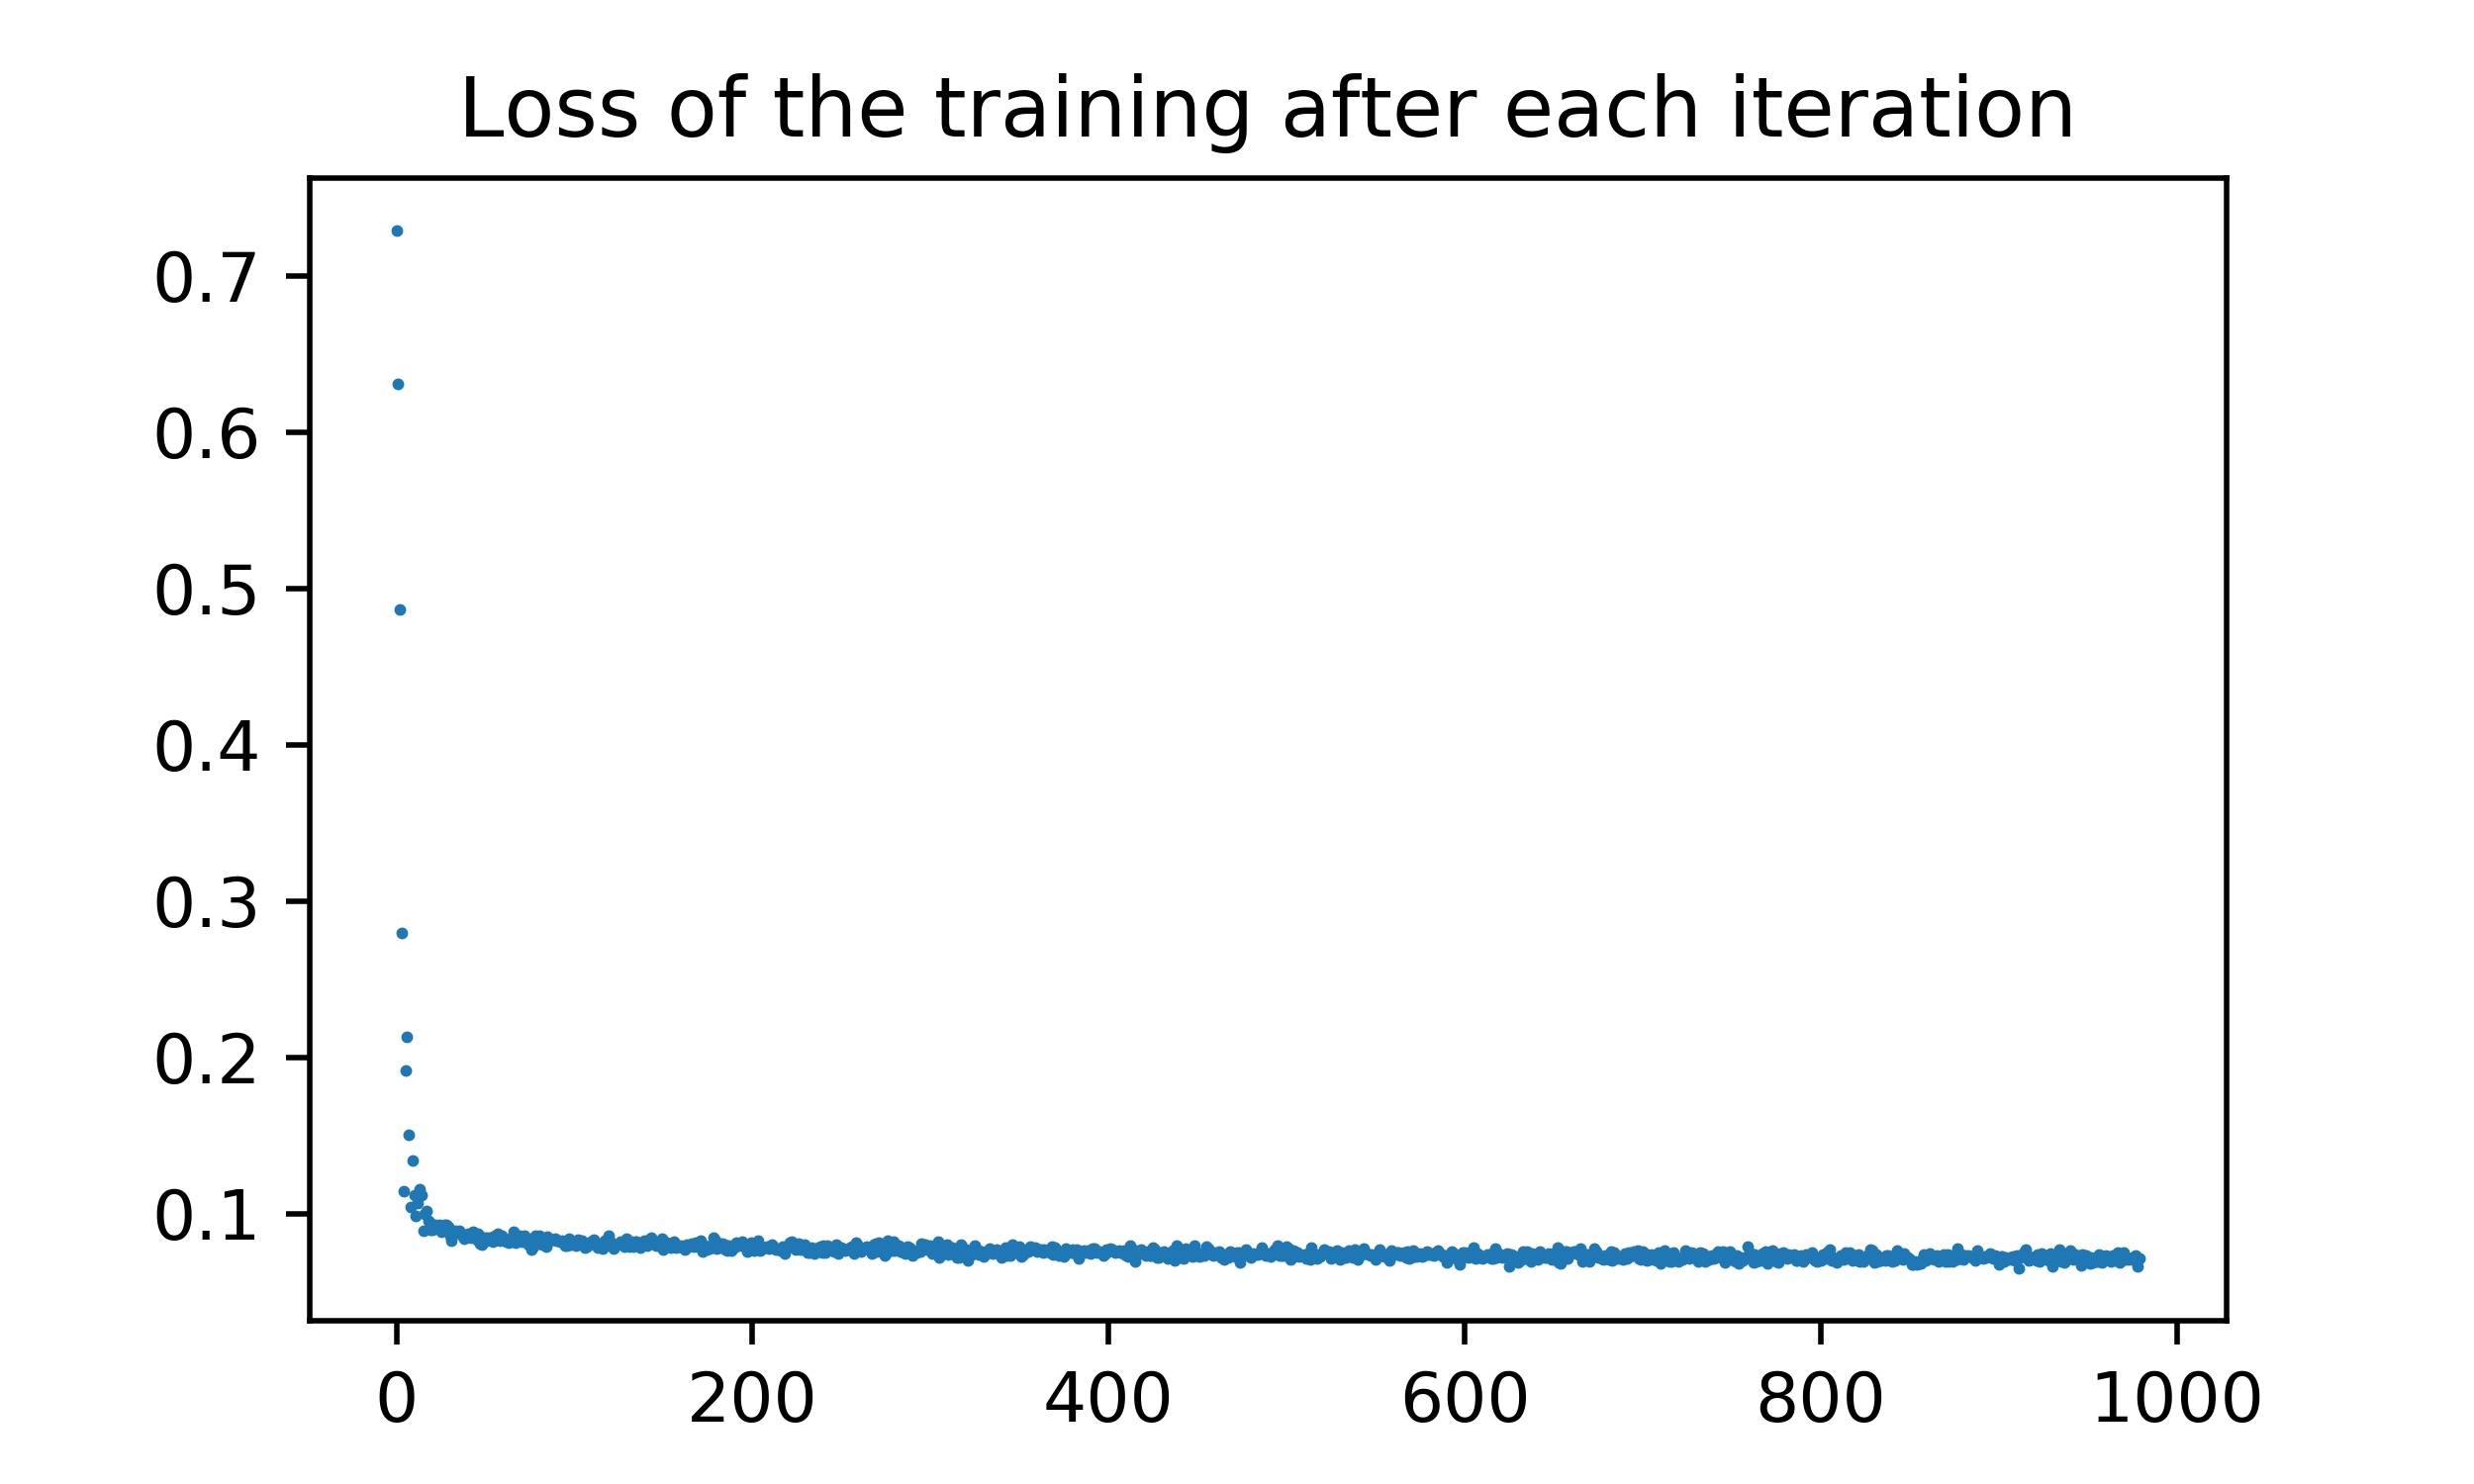
\includegraphics[width=0.5\textwidth]{alexnet-lazy-1_0-train-loss.png}
\caption{\label{alexnet:alexnet-lazy-1_0-loss}AlexNet loss plot with learning rate 0.01.}
\end{figure}

\begin{figure}[!ht]
\centering
\begin{subfigure}{.5\textwidth}
	\centering
	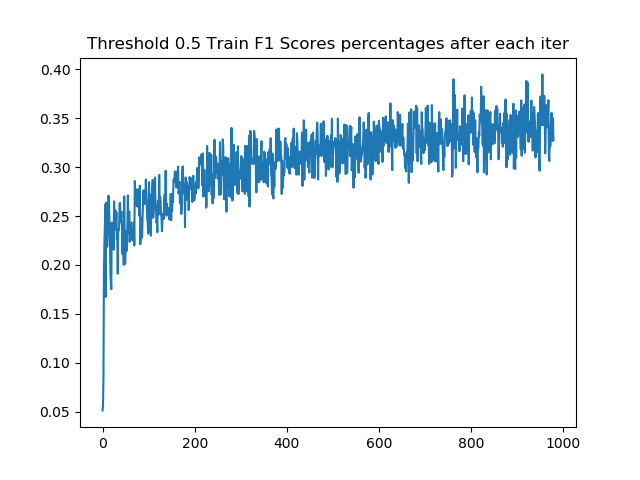
\includegraphics[width=1\linewidth]{alexnet-lazy-1_0-train-scores-f1-5.png}
	\caption{\label{alexnet:alexnet-lazy-1_0-train-scores-f1-5}AlexNet f1-score, threshold 0.5}
\end{subfigure}%
\begin{subfigure}{.5\textwidth}
	\centering
	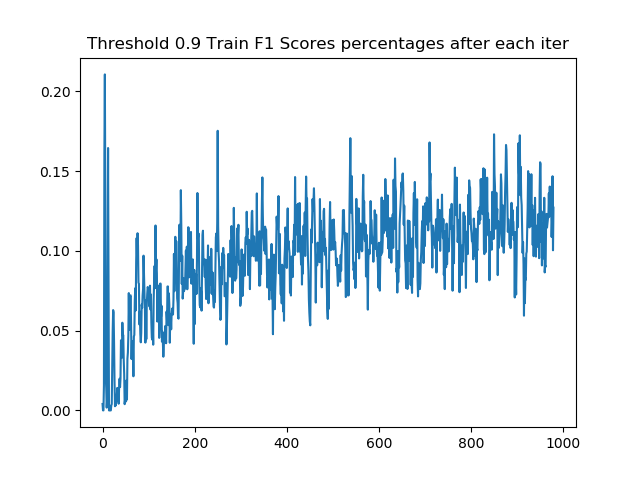
\includegraphics[width=1\linewidth]{alexnet-lazy-1_0-train-scores-f1-9.png}
	\caption{ \label{alexnet:alexnet-lazy-1_0-train-scores-f1-9}AlexNet f1-score, threshold 0.9}
\end{subfigure}
\end{figure}
\paragraph{}Loss decreases during training, however stuck at 0.6, f1-score increases and goes around \%30 between \%40 with 0.5 threshold. However threshold .9 gives really bad results. Hamming score is also increases and but goes around between \%20 and \%25.
\begin{figure}[!ht]
\centering
\begin{subfigure}{.5\textwidth}
	\centering
	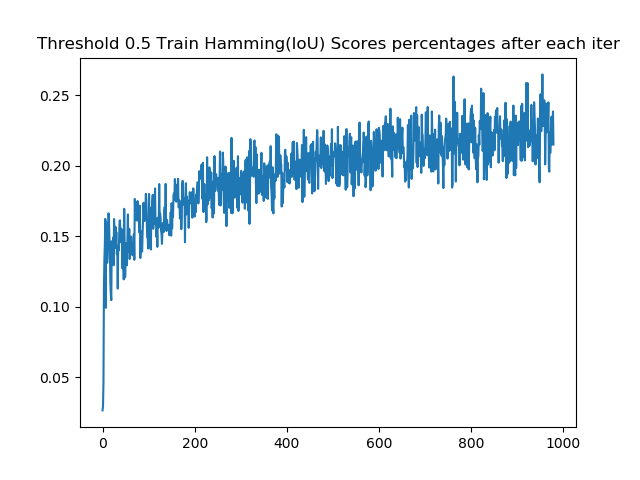
\includegraphics[width=1\linewidth]{alexnet-lazy-1_0-train-scores-hs-5.png}
	\caption{\label{alexnet:alexnet-lazy-1_0-train-scores-hs-5}AlexNet IoU score, threshold 0.5}
\end{subfigure}%
\begin{subfigure}{.5\textwidth}
	\centering
	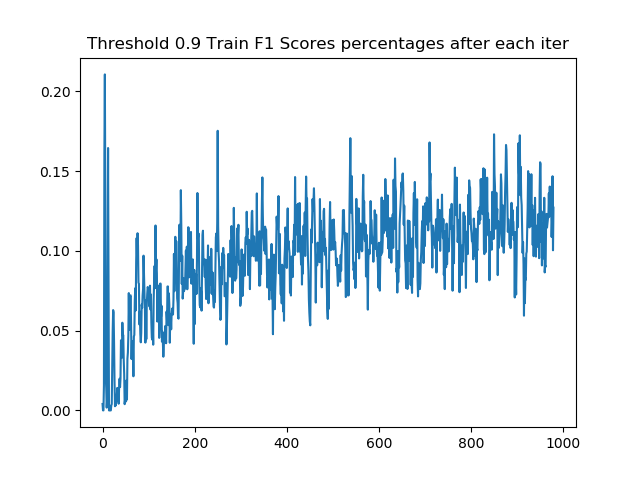
\includegraphics[width=1\linewidth]{alexnet-lazy-1_0-train-scores-f1-9.png}
	\caption{\label{alexnet:alexnet-lazy-1_0-train-scores-hs-9}AlexNet IoU score, threshold 0.9}
\end{subfigure}
\end{figure}

\begin{figure}[!ht]
\centering
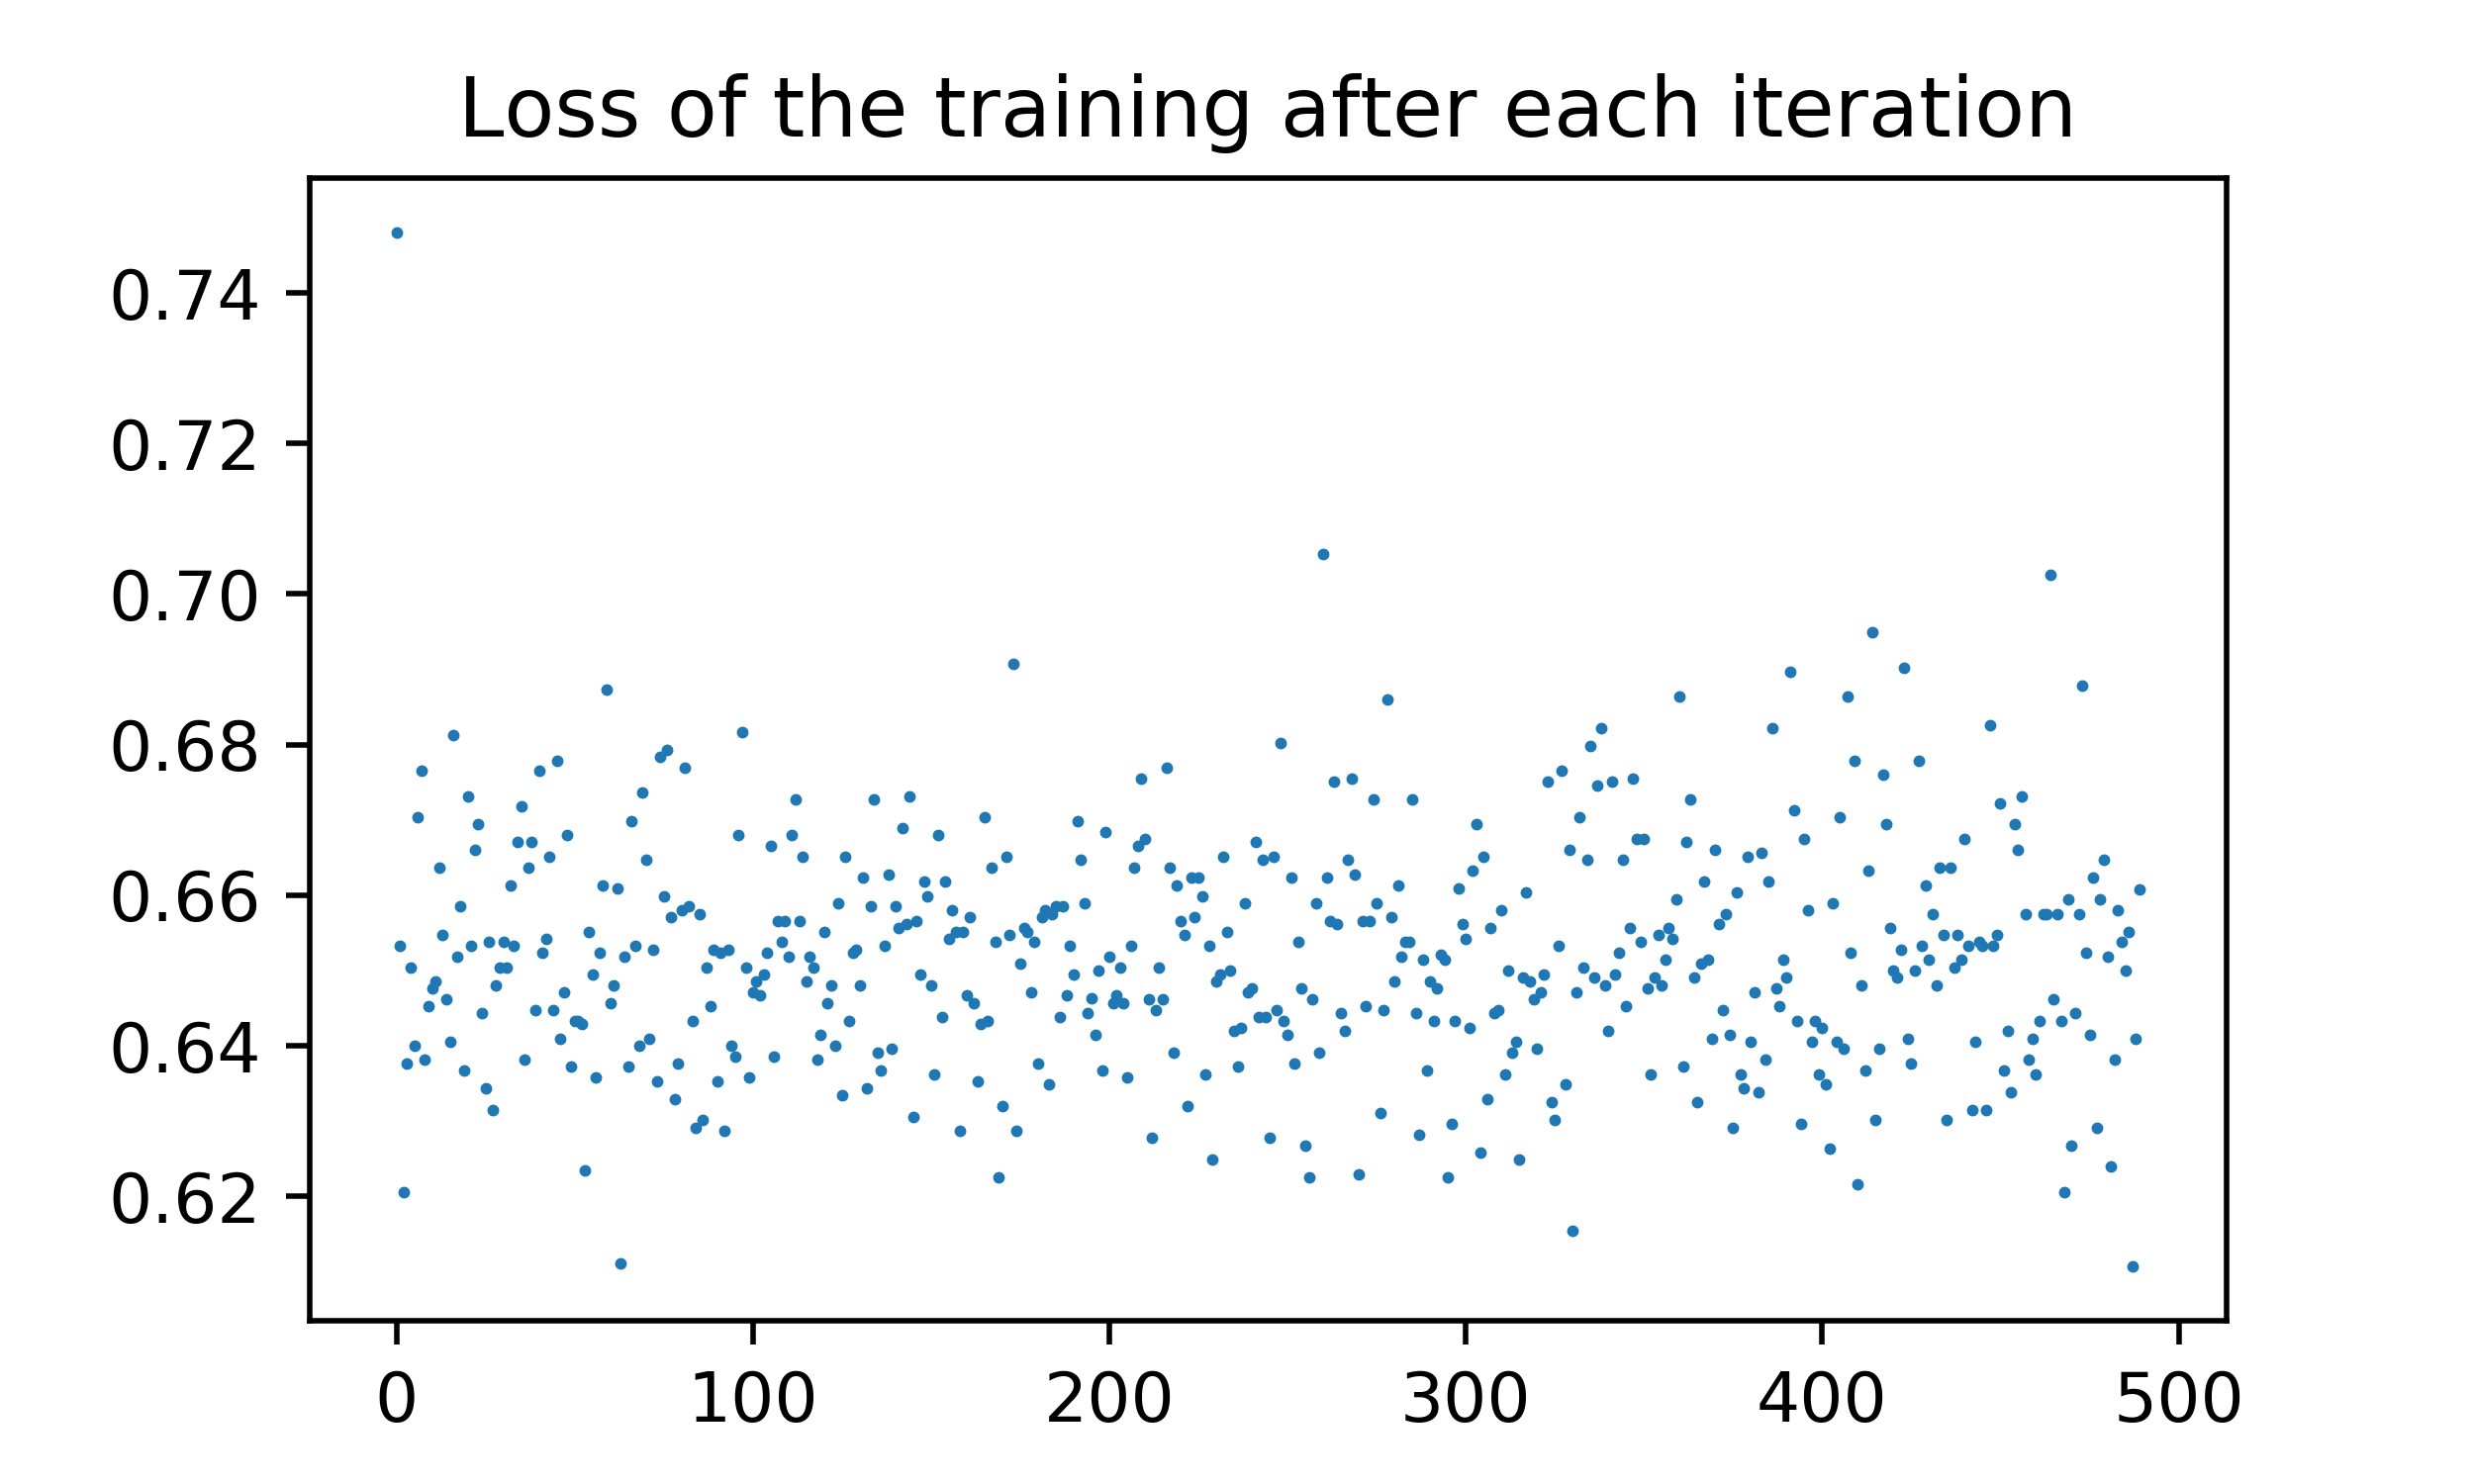
\includegraphics[width=0.5\textwidth]{alexnet-lazy-adam-1_0-train-loss.png}
\caption{\label{alexnet:alexnet-lazy-adam-1_0-train-loss}AlexNet loss plot with learning rate 0.01. with "Adam" optimizer}
\end{figure}

\begin{figure}[!ht]
\centering
\begin{subfigure}{.5\textwidth}
	\centering
	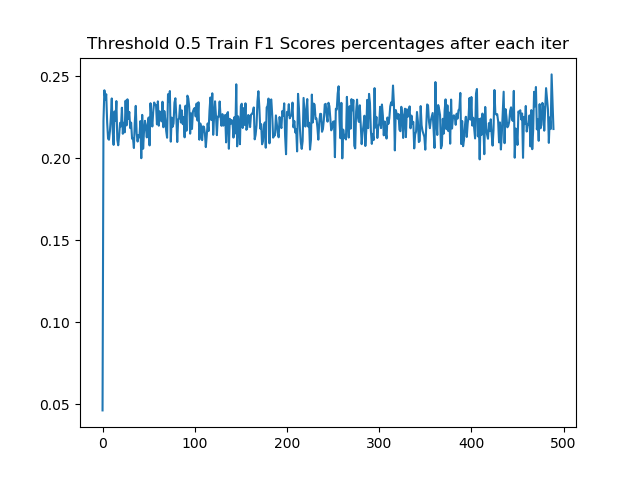
\includegraphics[width=1\linewidth]{alexnet-lazy-adam-1_0-train-scores-f1-5.png}
	\caption{\label{alexnet:alexnet-adam-lazy-1_0-train-scores-f1-5}AlexNet f1-score, threshold 0.5 with "Adam" optimizer}
\end{subfigure}%
\begin{subfigure}{.5\textwidth}
	\centering
	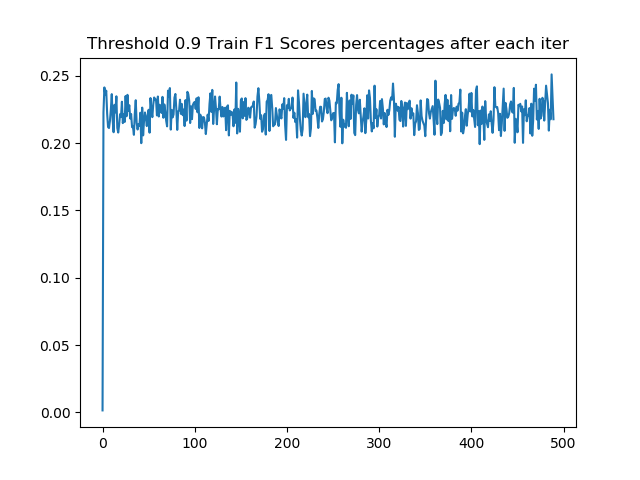
\includegraphics[width=1\linewidth]{alexnet-lazy-adam-1_0-train-scores-f1-9.png}
	\caption{\label{alexnet:alexnet-lazy-adam-1_0-train-scores-f1-9}AlexNet f1-score, threshold 0.9 with "Adam" optimizer}
\end{subfigure}
\end{figure}
\paragraph{}AlexNet is with Adam optimizer does not give stable loss. Also it gives good scores suddenly however then stuck at that point just like behaves it has big learning rate.
\begin{figure}[!ht]
\centering
\begin{subfigure}{.5\textwidth}
	\centering
	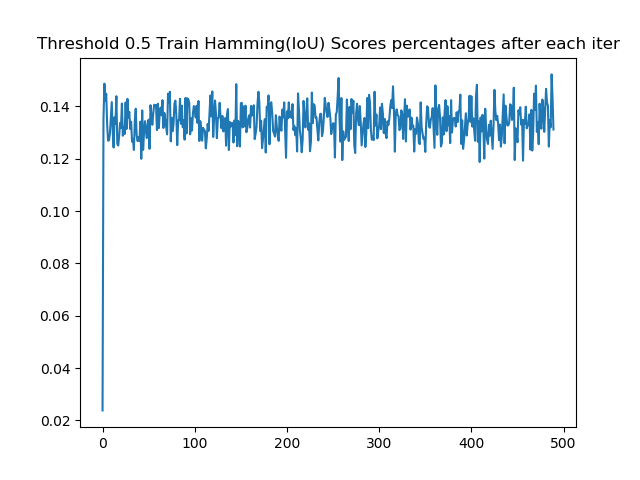
\includegraphics[width=1\linewidth]{alexnet-lazy-adam-1_0-train-scores-hs-5.png}
	\caption{\label{alexnet:alexnet-lazy-adam-1_0-train-scores-hs-5}AlexNet IoU score, threshold 0.5 with "Adam" optimizer}
\end{subfigure}%
\begin{subfigure}{.5\textwidth}
	\centering
	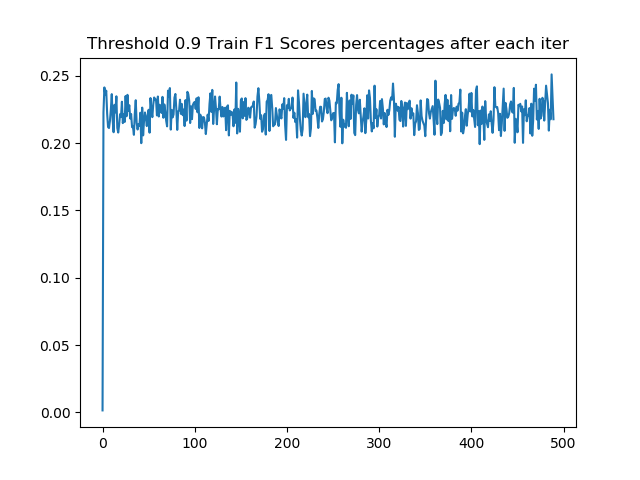
\includegraphics[width=1\linewidth]{alexnet-lazy-adam-1_0-train-scores-f1-9.png}
	\caption{\label{alexnet:alexnet-lazy-adam-1_0-train-scores-hs-9}AlexNet IoU score, threshold 0.9 with "Adam" optimizer} 
\end{subfigure}
\end{figure}

\begin{figure}[!ht]
\centering
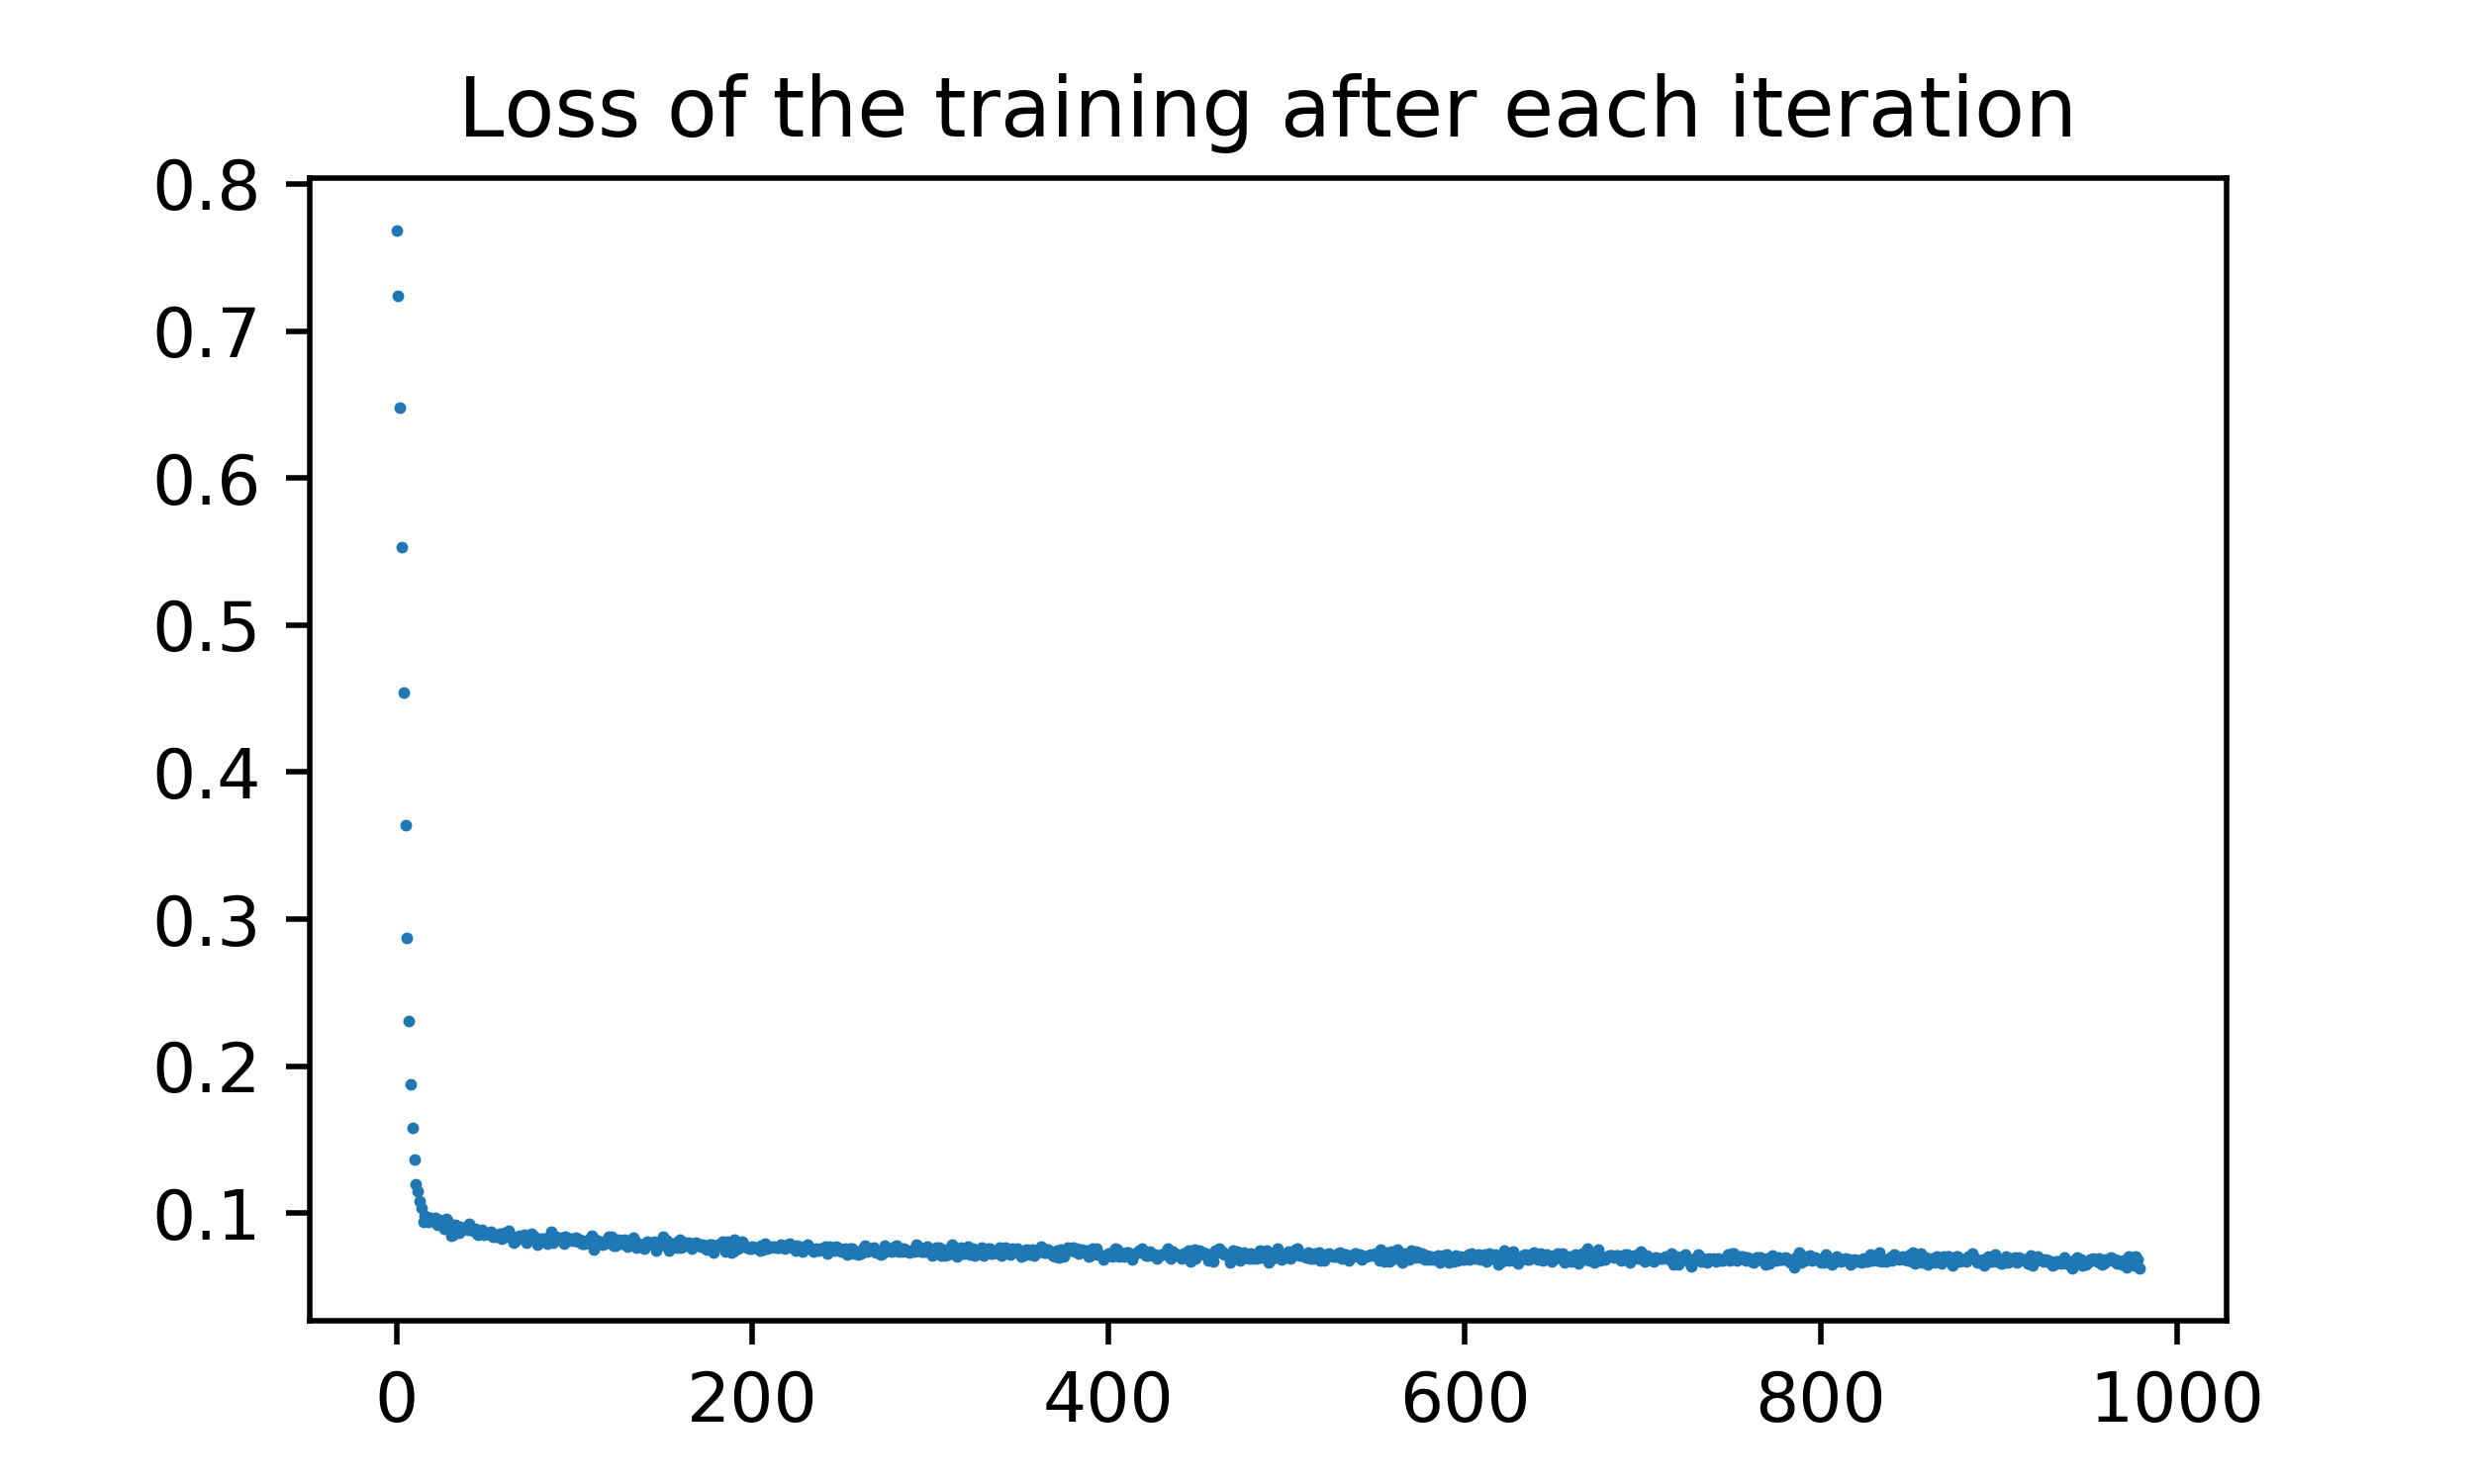
\includegraphics[width=0.5\textwidth]{resnet18-lazy-1_0-train-loss.png}
\caption{\label{resnet18:resnet18-lazy-1_0-train-loss}ResNet loss plot with learning rate 0.01.}
\end{figure}

\begin{figure}[!ht]
\centering
\begin{subfigure}{.5\textwidth}
	\centering
	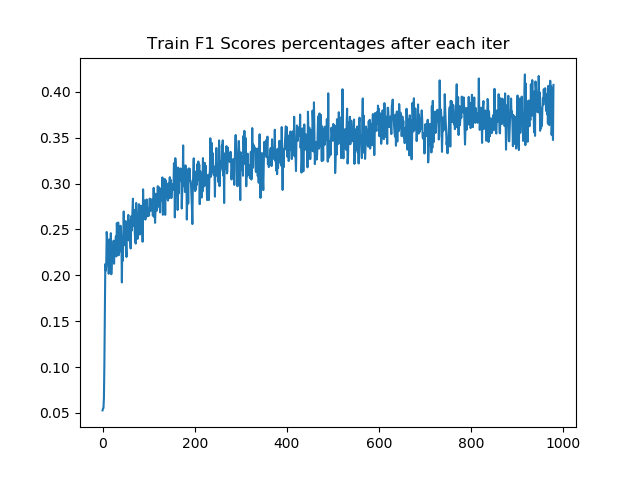
\includegraphics[width=1\linewidth]{resnet18-lazy-1_0-train-scores-f1.png}
	\caption{\label{resnet18:resnet18-lazy-1.0-train-scores-f1}ResNet18 f1-score, threshold 0.5}
\end{subfigure}%
\begin{subfigure}{.5\textwidth}
	\centering
	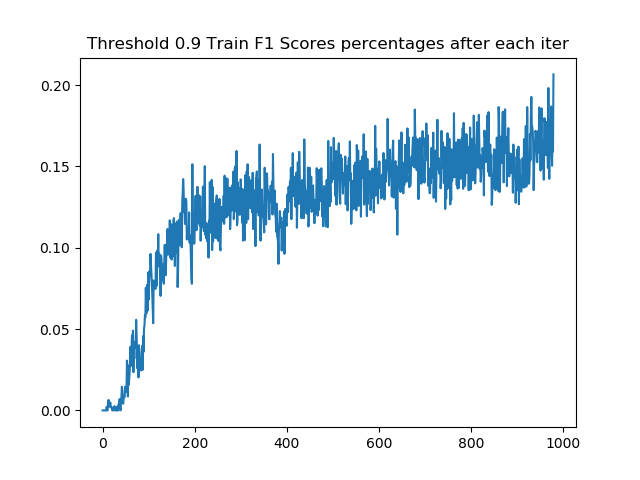
\includegraphics[width=1\linewidth]{resnet18-lazy-1_0-train-scores-f1-9.png}
	\caption{\label{resnet18:resnet18-lazy-1.0-train-scores-f1-9}ResNet18 f1-score, threshold 0.9}
\end{subfigure}
\end{figure}
\paragraph{}ResNet18 has similar loss plot like AlexNet with SGD in Figure \ref{resnet18:resnet18-lazy-1_0-train-loss}, f1-score and hamming score increases more stabilized than AlexNet, and gives slightly better scores. 
\begin{figure}[!ht]
\centering
\begin{subfigure}{.5\textwidth}
	\centering
	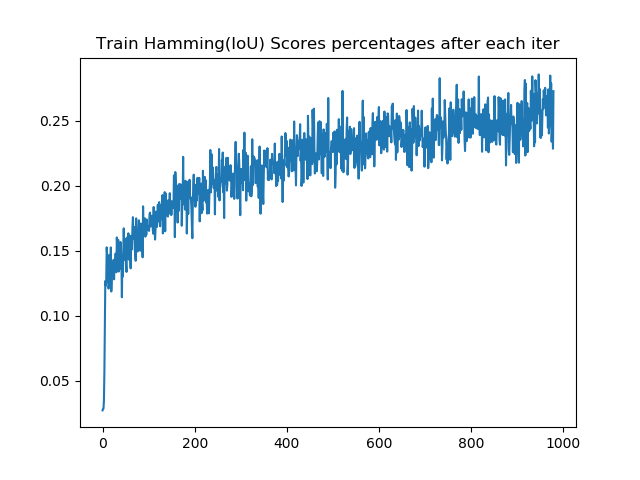
\includegraphics[width=1\linewidth]{resnet18-lazy-1_0-train-scores-hs.png}
	\caption{ \label{resnet18:resnet18-lazy-1.0-train-scores-hs-5}ResNet18 IoU score, threshold 0.5}
\end{subfigure}%
\begin{subfigure}{.5\textwidth}
	\centering
	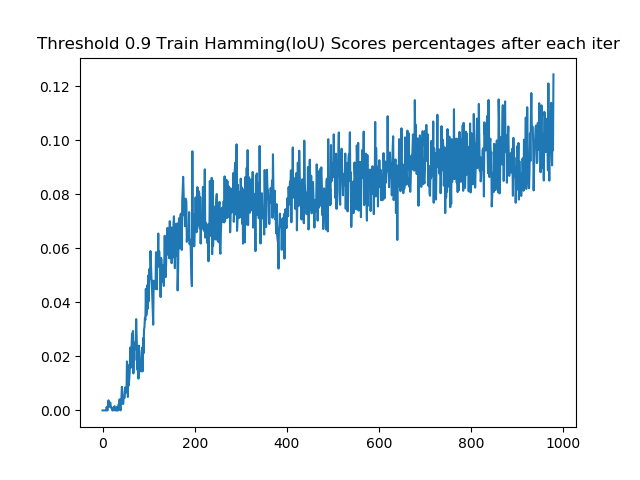
\includegraphics[width=1\linewidth]{resnet18-lazy-1_0-train-scores-hs-9.png}
	\caption{\label{resnet18:resnet18-lazy-1.0-train-scores-hs-9}ResNet18 IoU score, threshold 0.9}
\end{subfigure}
\end{figure}

\begin{figure}[!ht]
\centering
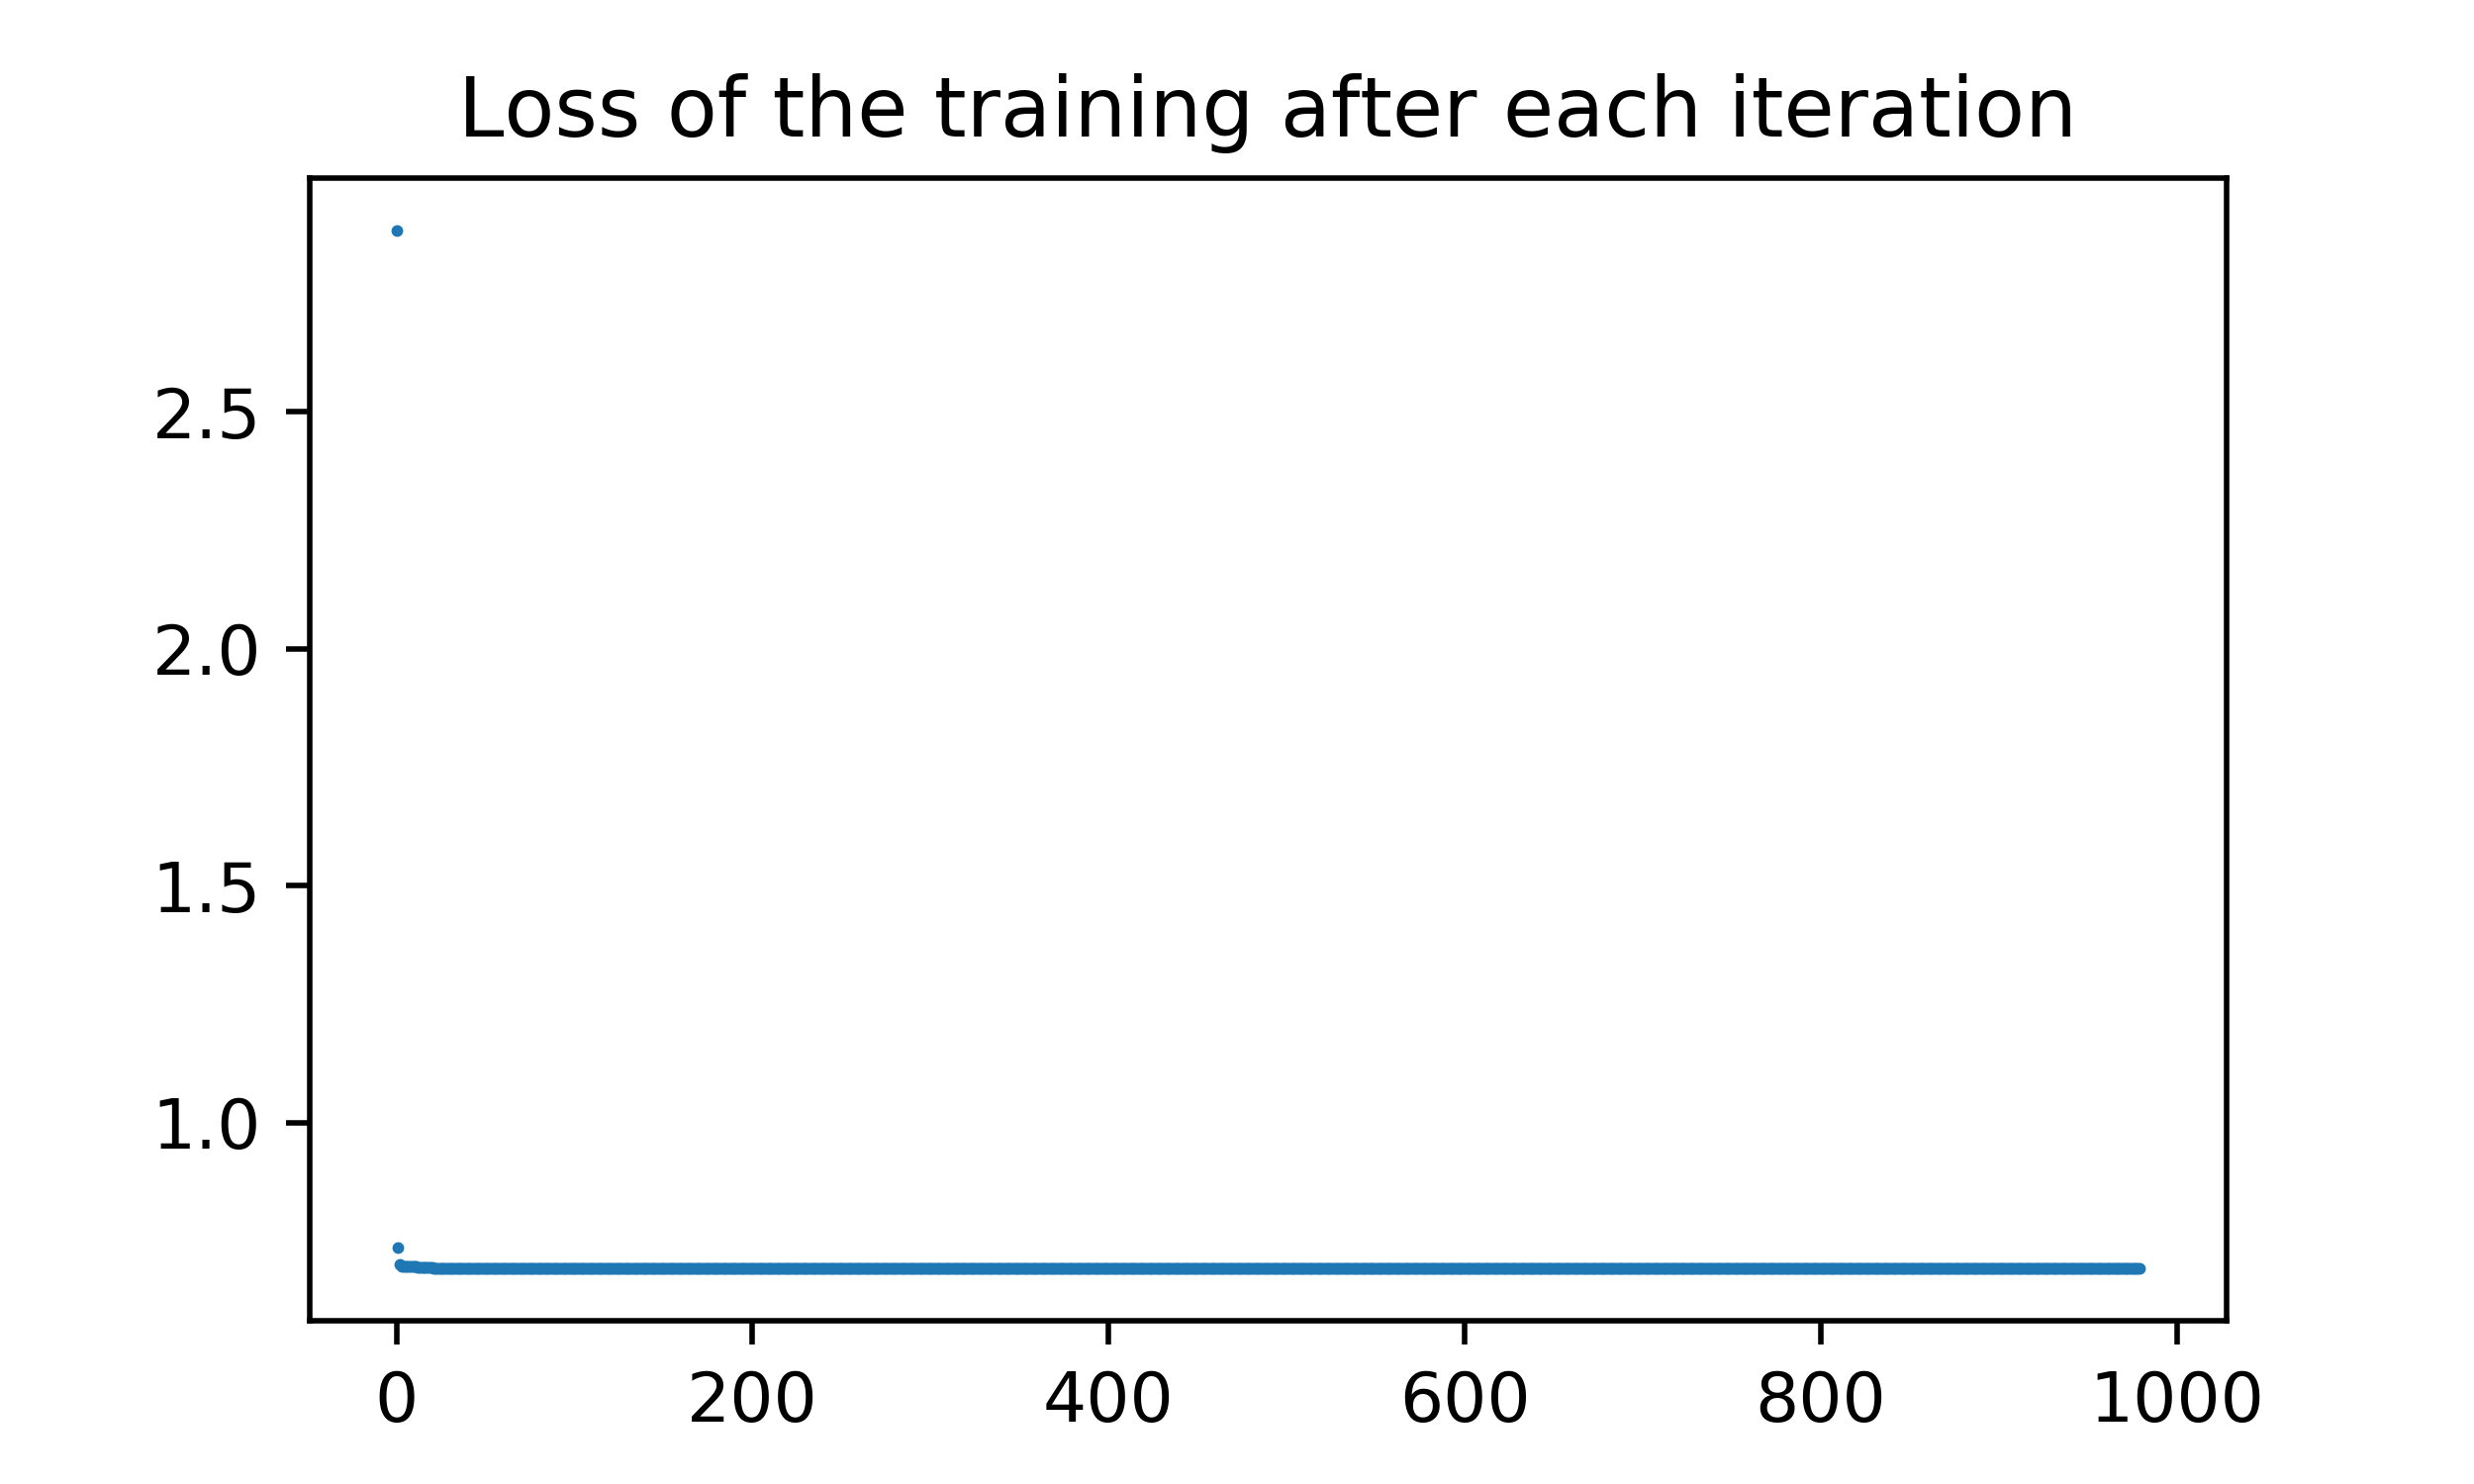
\includegraphics[width=0.5\textwidth]{squeezenet-lazy-1-train-loss.png}
\caption{\label{squeezenet:squeezenet-lazy-1-train-loss}SqueezeNet loss plot with learning rate 0.01.}
\end{figure}

\begin{figure}[!ht]
\centering
\begin{subfigure}{.5\textwidth}
	\centering
	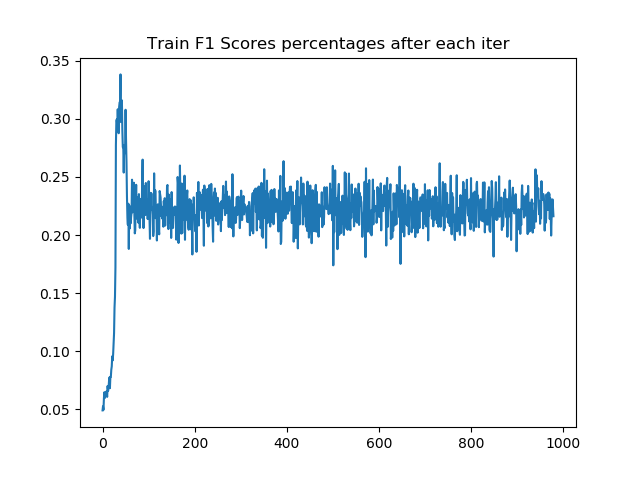
\includegraphics[width=1\linewidth]{squeezenet-lazy-1-train-scores-f1.png}
	\caption{\label{squeezenet:squeezenet-lazy-1-train-scores-f1}SqueezeNet f1-score, threshold 0.5}
\end{subfigure}%
\begin{subfigure}{.5\textwidth}
	\centering
	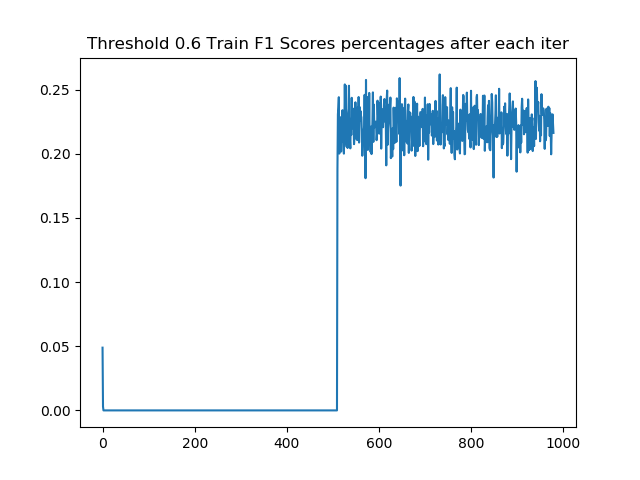
\includegraphics[width=1\linewidth]{squeezenet-lazy-1-train-scores-f1-6.png}
	\caption{\label{squeezenet:squeezenet-lazy-1-train-scores-f1-6}SqueezeNet f1-score, threshold 0.6}
\end{subfigure}
\end{figure}
\paragraph{}SqueezeNet is clearly worst of them. Loss is stuck badly in Figure \ref{squeezenet:squeezenet-lazy-1-train-loss} and thresholds behave differently from each other. In threshold 0.5, it stuck after some epoch and it does not learn anything. However in the case of threshold 0.6, it does not give any result at some point. After some epoch score increase suddenly however it stuck again. In threshold 0.7, it is worst, there are no result. 
\begin{figure}[!ht]
\centering
\begin{subfigure}{.5\textwidth}
	\centering
	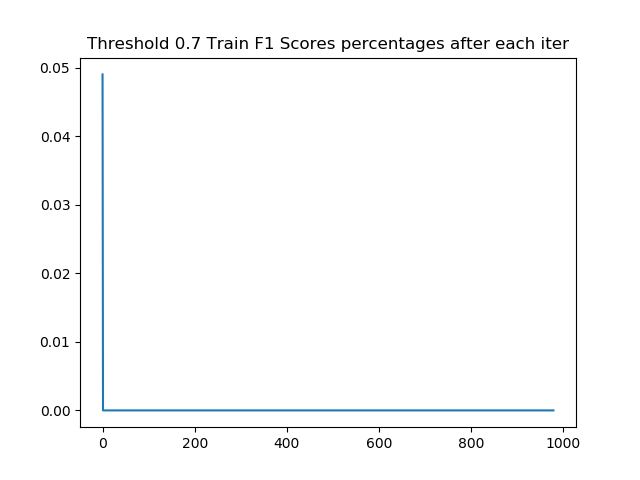
\includegraphics[width=.9\linewidth]{squeezenet-lazy-1-train-scores-f1-7.png}
	\caption{\label{squeezenet:squeezenet-lazy-1-train-scores-f1-7}SqueezeNet f1-score, threshold 0.7}
\end{subfigure}%
\begin{subfigure}{.5\textwidth}
	\centering
	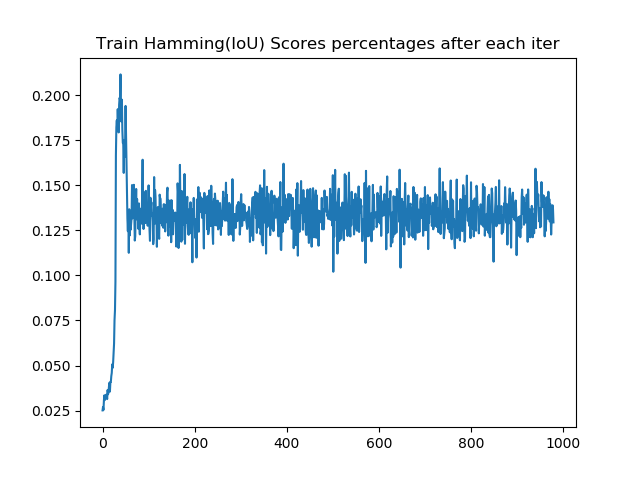
\includegraphics[width=.9\linewidth]{squeezenet-lazy-1-train-scores-hs.png}
	\caption{\label{squeezenet:squeezenet-lazy-1-train-scores-hs}SqueezeNet IoU score, threshold 0.5}
\end{subfigure}
\end{figure}

\begin{figure}[!ht]
\centering
\begin{subfigure}{.5\textwidth}
	\centering
	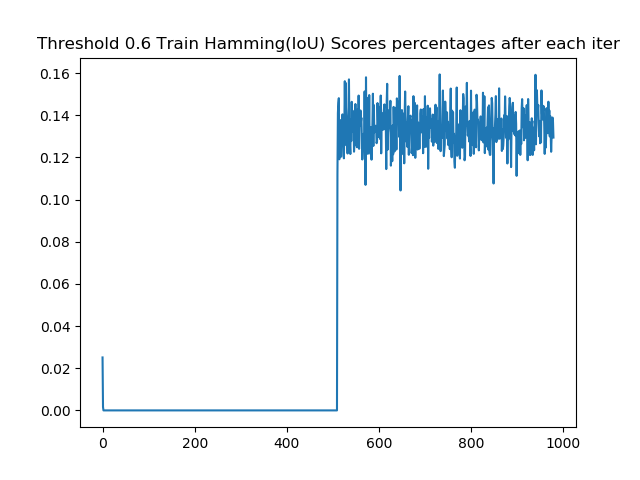
\includegraphics[width=0.9\linewidth]{squeezenet-lazy-1-train-scores-hs-6.png}
	\caption{\label{squeezenet:squeezenet-lazy-1-train-scores-hs-6}SqueezeNet IoU score, threshold 0.6}
\end{subfigure}%
\begin{subfigure}{.5\textwidth}
	\centering
	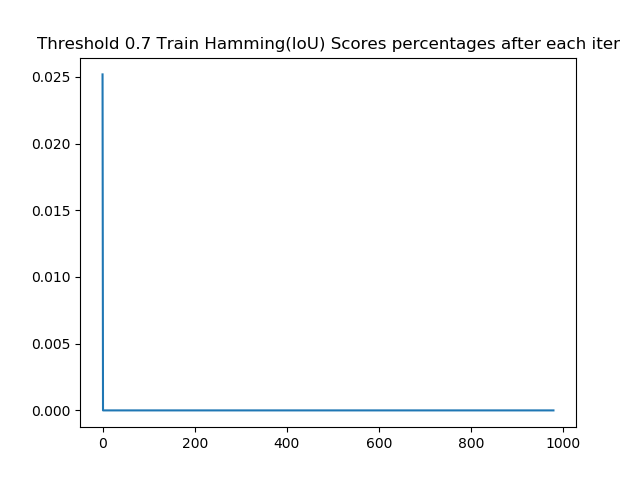
\includegraphics[width=0.9\linewidth]{squeezenet-lazy-1-train-scores-hs-7.png}
	\caption{\label{squeezenet:squeezenet-lazy-1-train-scores-hs-7}SqueezeNet IoU score, threshold 0.7}
\end{subfigure}
\end{figure}

\begin{figure}[!ht]
\centering
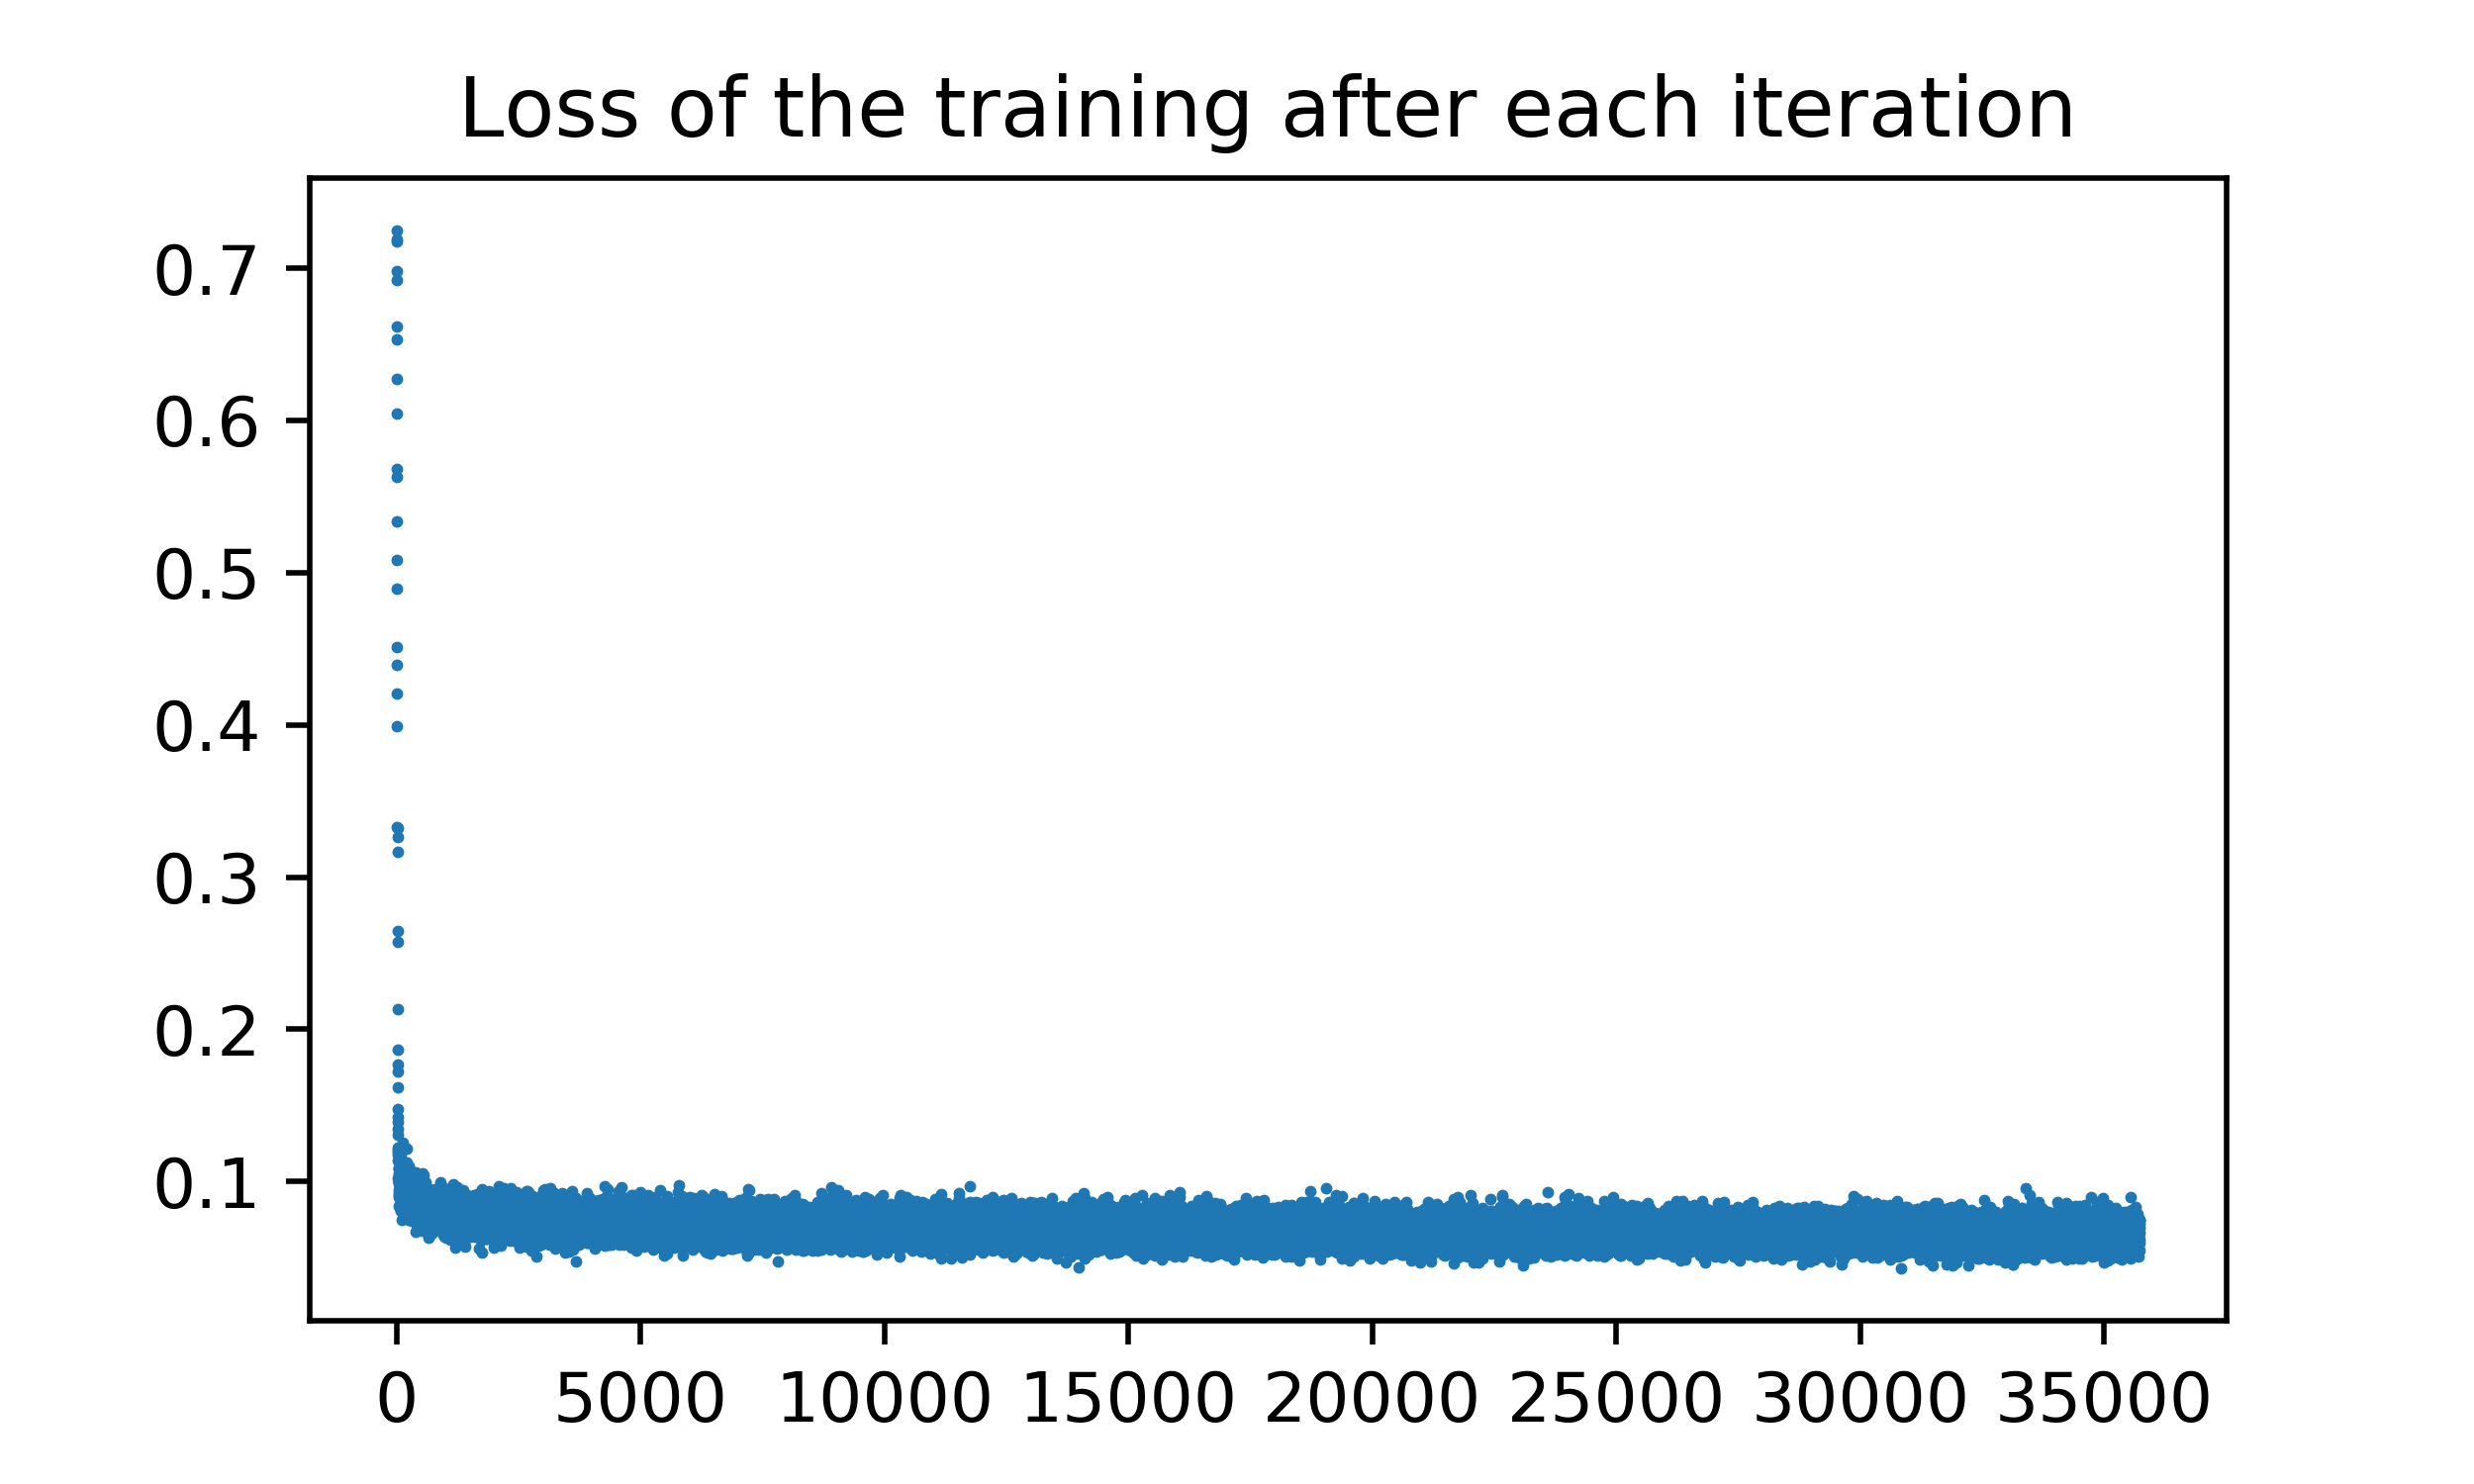
\includegraphics[width=0.5\textwidth]{vgg16-0_26-lazy-1-train-loss.png}
\caption{\label{vgg16:vgg16-ft-train-loss}freezing VGG16 loss plot}
\end{figure}

\begin{figure}[!ht]
\centering
\begin{subfigure}{.5\textwidth}
	\centering
	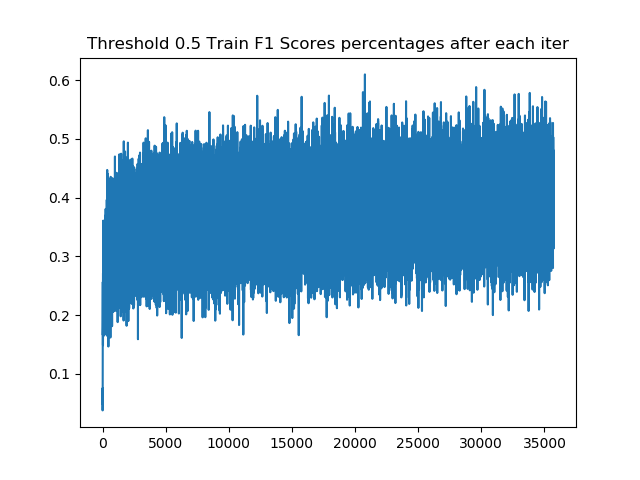
\includegraphics[width=1\linewidth]{vgg16-0_26-lazy-1-train-scores-f1-5.png}
	\caption{\label{vgg16:vgg16-0_26-lazy-1-train-scores-f1-5}freezing VGG16 f1-score, threshold 0.5}
\end{subfigure}%
\begin{subfigure}{.5\textwidth}
	\centering
	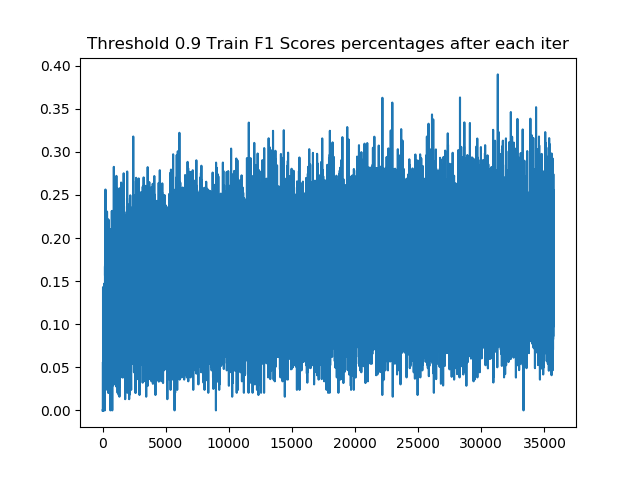
\includegraphics[width=1\linewidth]{vgg16-0_26-lazy-1-train-scores-f1-9.png}
	\caption{\label{vgg16:vgg16-0_26-lazy-1-train-scores-f1-9}freezing VGG16 f1-score, threshold 0.9}
\end{subfigure}
\end{figure}

\paragraph{}VGG16 is really huge model, it is fine-tuned firstly. It converges slower than non-freezing version of VGG16. Little batches are used in training, that is why there is so many iterations in epochs. threshold 0.5 gives best results. Even it is reaches \%60, generally there are many up and downs, it gives \%40 F1 scores overall. Hamming score has \%20 overall.   

\begin{figure}[!ht]
\centering
\begin{subfigure}{.5\textwidth}
	\centering
	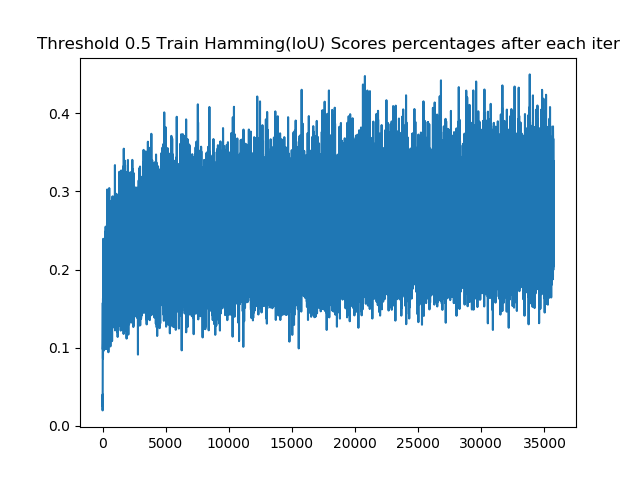
\includegraphics[width=1\linewidth]{vgg16-0_26-lazy-1-train-scores-hs-5.png}
	\caption{\label{vgg16:vgg16-0_26-lazy-1-train-scores-hs-5}freezing VGG16 IoU score, threshold 0.5}
\end{subfigure}%
\begin{subfigure}{.5\textwidth}
	\centering
	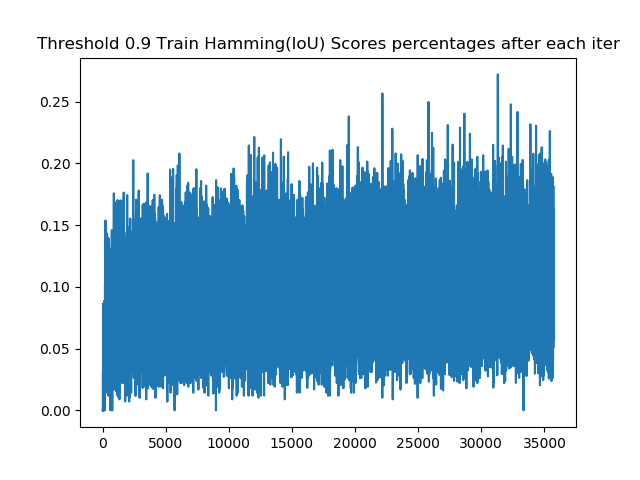
\includegraphics[width=1\linewidth]{vgg16-0_26-lazy-1-train-scores-hs-9.png}
	\caption{\label{vgg16:vgg16-0_26-lazy-1-train-scores-hs-9}freezing VGG16 IoU, threshold 0.9}
\end{subfigure}
\end{figure}

\begin{figure}[!ht]
\centering
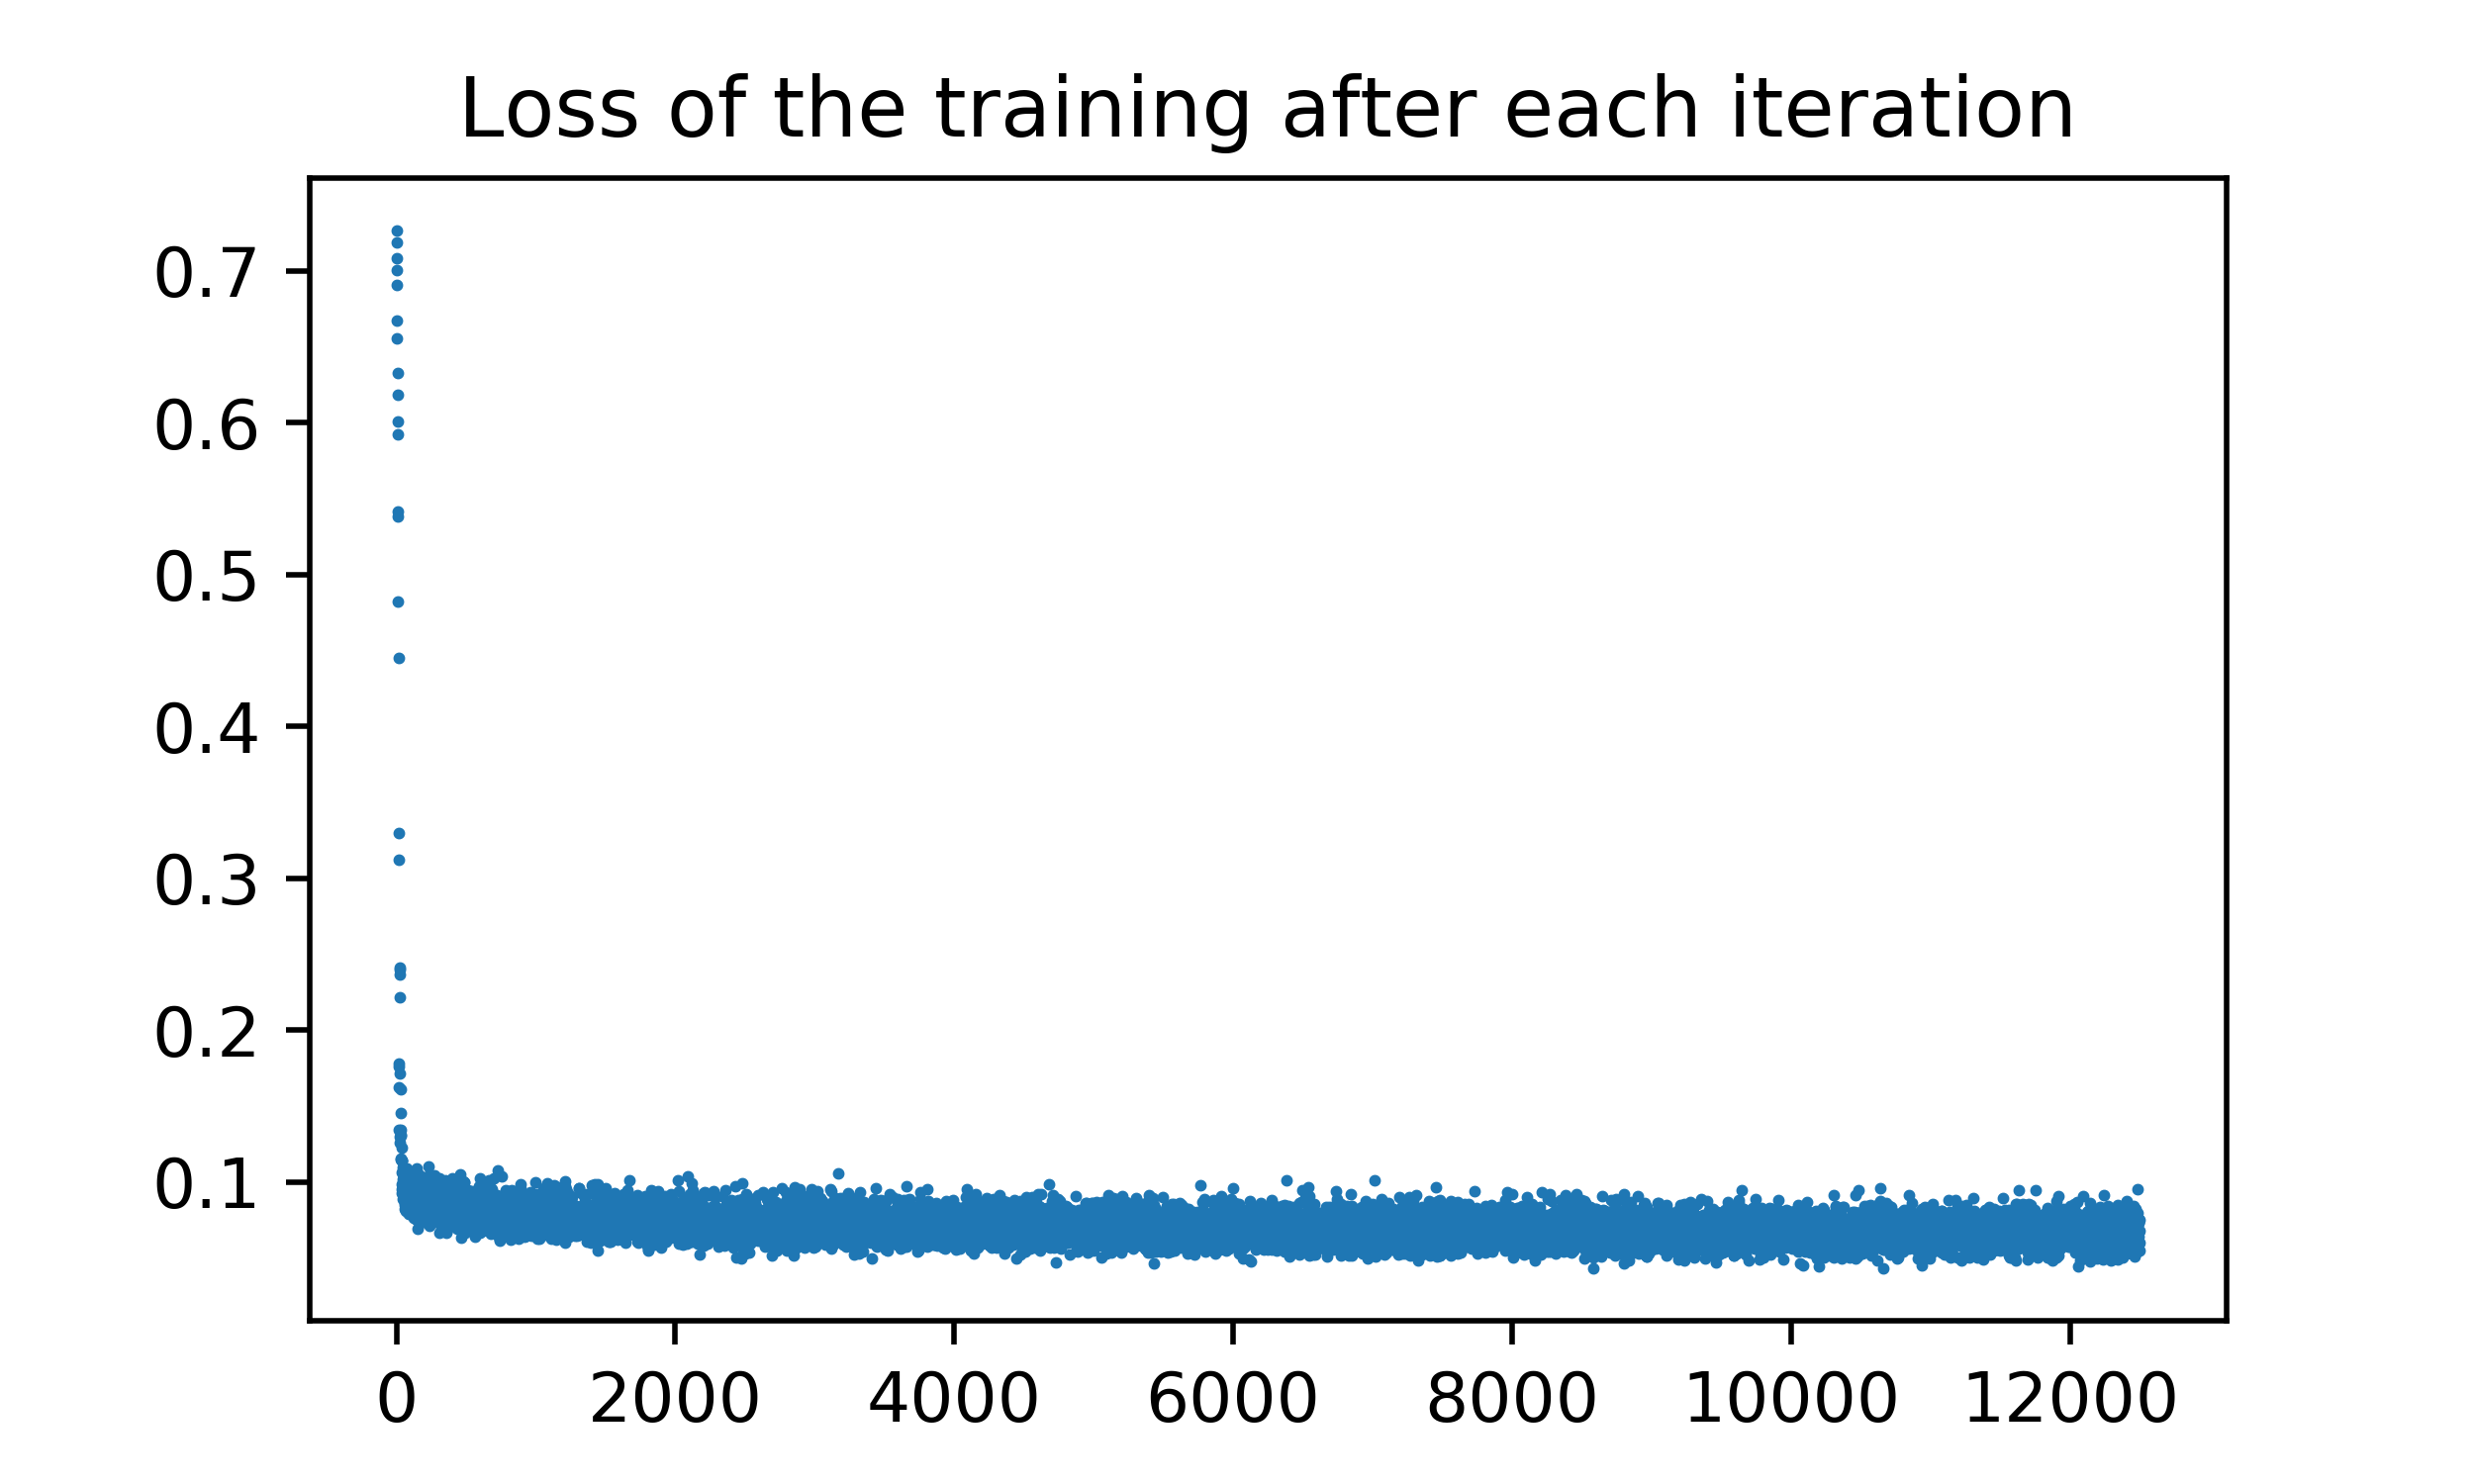
\includegraphics[width=0.5\textwidth]{vgg16-full-lazy-1-train-loss.png}
\caption{\label{vgg16:vgg16-full-train-loss}VGG16 loss plot}
\end{figure}

\begin{figure}[!ht]
\centering
\begin{subfigure}{.5\textwidth}
	\centering
	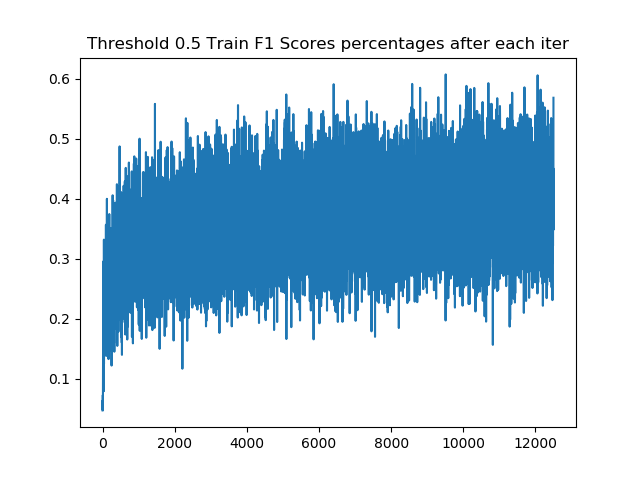
\includegraphics[width=1\linewidth]{vgg16-full-lazy-1-train-scores-f1-5.png}
	\caption{\label{vgg16:vgg16-full-lazy-1-train-scores-f1-5}VGG16 f1-score, threshold 0.5}
\end{subfigure}%
\begin{subfigure}{.5\textwidth}
	\centering
	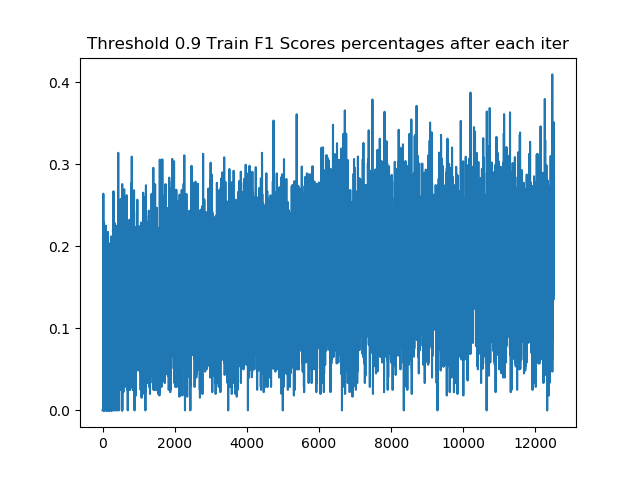
\includegraphics[width=1\linewidth]{vgg16-full-lazy-1-train-scores-f1-9.png}
	\caption{\label{vgg16:vgg16-full-lazy-1-train-scores-f1-9}VGG16 f1-score, threshold 0.9}
\end{subfigure}
\end{figure}

\paragraph{}After using layer freezing on VGG16, we trained non-freezing pre-trained VGG16. It convergences faster, however it is slightly better and has many ups and downs, too. Therefore, we can say that it is slightly better than others.

\begin{figure}[!ht]
\centering
\begin{subfigure}{.5\textwidth}
	\centering
	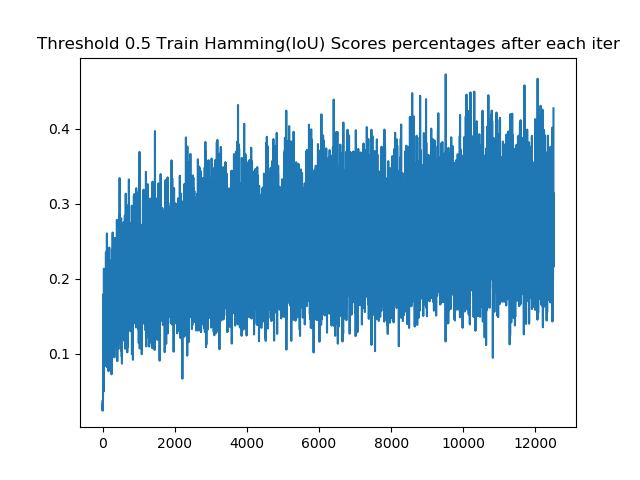
\includegraphics[width=1\linewidth]{vgg16-full-lazy-1-train-scores-hs-5.png}
	\caption{\label{vgg16:vgg16-full-lazy-1-train-scores-hs-5}VGG16 IoU score, threshold 0.5}
\end{subfigure}%
\begin{subfigure}{.5\textwidth}
	\centering
	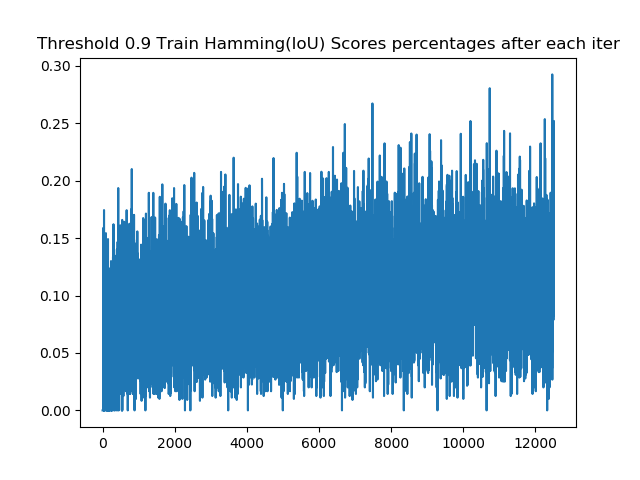
\includegraphics[width=1\linewidth]{vgg16-full-lazy-1-train-scores-hs-9.png}
	\caption{\label{vgg16:vgg16-full-lazy-1-train-scores-hs-9}VGG16 IoU, threshold 0.9}
\end{subfigure}
\end{figure}

\section{Discussion}
\paragraph{}As mentioned before, those results are satisfactory. We expected at least \%70-\%80 in training scores. One of the reason why it did not happened to be those kind of scores is to probably stuck at some local-maxima point. However, we tried different learning rates, optimizer. Actually, if we use adam optimizer or another different optimizer on VGG16, things could be different however we do not have that kind of memory. Transfer learning could be solution of this problem. Besides, using SVM on top of models that would be used for feature extraction in this case could be another solution because SVM finds always global minimum in its case. Also, for this dataset different approaches should be taken into account. Because, original dataset has about 1 million images and it has enough variance. However, for this kind of unbalanced dataset, model has really great bias while having low variance. We should have used preprocessing techniques or studied different techniques.  
\paragraph{}Another thing could be done is finding threshold for all labels instead of global threshold. It is actually implemented, but we could not try for analysis. In our implementation, we tried thresholds 0.1 to 0.9 with step size 0.1, then after applying this threshold to predictions calculates Matthews correlation coefficient which is a measure of the quality of binary classifications.\cite{matcof} It takes into account true and false positives and negatives and is generally regarded as a balanced measure which can be used even if the classes are of very different sizes. 
\paragraph{} As a result, there are many machine learning and computer vision solutions and techniques to be applied on this problem as we discussed before. Therefore using CNNs is one the possible easiest and effective solution, even though it needs many resources.  
\begin{thebibliography}{1} 
\bibitem{alexnet} Krizhevsky, A.\ 2014, arXiv:1404.5997 
\bibitem{squeezenet} Iandola, F.~N., Han, S., Moskewicz, M.~W., et al.\ 2016, arXiv:1602.07360 
 
\bibitem{imageNet} Deng, J. and Dong, W. and Socher, R. and Li, L.-J. and Li, K. and Fei-Fei, L., ImageNet: A Large-Scale Hierarchical Image Database, 2009 

\bibitem{vggNet} Karen Simonyan and Andrew Zisserman, Very Deep Convolutional Networks for Large-Scale Image Recognition, 2014 

\bibitem{resnet} He, K., Zhang, X., Ren, S., \& Sun, J.\ 2015, arXiv:1512.03385 
 
\bibitem{torchmodels} 
torch.models,
\\\texttt{http://pytorch.org/docs/master/torchvision/models.html}, Last-Accessed: \today{}

\bibitem{matcof}Matthews correlation coefficient,
\\\texttt{http://scikit-learn.org/stable/modules/generated/sklearn.metrics.matthews\_corrcoef.html}, Last-Accessed: \today{}
\end{thebibliography}


\end{document}
